\documentclass[12pt]{ctexart} 
\usepackage{array}
\usepackage{geometry}  
\usepackage{graphicx}  
\usepackage{amsmath, amssymb}  
\usepackage{booktabs}  
\usepackage{enumerate} 
\usepackage{verbatim}
\usepackage{url}
\usepackage{fancyhdr}  % 引入 fancyhdr 包
\pagestyle{fancy}  % 使用 fancy 页眉页脚样式
\fancyhf{}  % 清空默认的页眉页脚
\fancyfoot[C]{\thepage}  % 在底部中央显示页码
\renewcommand{\headrulewidth}{0pt}  % 去掉页眉的横线
%\pagestyle{empty}  % 去掉页眉和页脚的页码
% 页面设置  
\geometry{a4paper, margin=2.5cm}  
\setlength{\parindent}{2em} % 2em 相当于两个字符的宽度

%\title{基于收益最大化的种植策略探究}  
%\author{张文瑞、陈名湛、王晨屹}  
%\date{\today}  

\begin{document}  
%	\maketitle  
	
	% 摘要页  
	%\newpage 
	\section*{基于收益最大化的种植策略研究} 
	%\title{基于收益最大化的种植策略探究}
	\begin{center}  
		\Large\textbf{摘要}  
	\end{center}  
	
	\noindent   
	
	
	随着乡村振兴战略的实施,使农作物收益最大化具有重要意义。同时随着市场需求的改变,农产品销售面临诸多潜在风险。本文从如何使农产品收益最大化出发,根据需求变化灵活选取不同的约束条件和求解算法,设计不同的农作物种植结构,以达到充分利用耕地资源的目的。
	
	
	针对问题一,我们首先对不同作物亩产收益进行分析,发现种植豆类的收益低于种植蔬菜与粮食,因此我们提出了种植豆类收益低的假设。在此假设基础上,本文建立\textbf{单目标多约束优化模型},以农作物种植收益作为目标函数,考虑到题目中的约束函数多为非线性约束,因此常规的线性规划算法不容易实现,因此我们基于\textbf{遗传算法}的相关思想,针对种植策略的有效性和高收益性进行全局优化,通过反复迭代得到了在该题约束下最优的种植策略。
	
	
	针对问题二,由于诸多变量发生波动,若继续设计常规的单目标规划模型容易造成较大误差。因此本文采用\textbf{概率规划模型},利用经济学中的\textbf{几何布朗运动模型}将价格随时间变化的随机过程转化为微分方程形式,再利用\textbf{对数收益的正态分布模型}模拟价格的变化,使其在一定取值范围内满足正态分布,接着通过重复模拟收益生成路径得到了农作物在不同年份收益的期望值分布列。考虑到潜在的种植风险,本文引入了\textbf{在险价值}来模拟可能出现的最大损失。最后,考虑到不确定因素下集合的选取问题可能会对优化过程产生较大影响,本文采用了\textbf{鲁棒优化模型},并重新设计了目标函数与约束条件,进而得出了本题的最佳优化种植结构:单季地以种植红薯为主。水浇地奇数年第一季主要种植茄子和豇豆,第二季全部种植水稻,偶数年第一季全部种植茄子,第二季种植水稻。
	
	
	针对问题三,本文计算\textbf{speraman相关系数}分析各作物预期销售量,种植成本,销售价格之间的关系,结果表明亩产量与种植成本之间具有较强的正相关性,平均销售单价与种植成本之间存在弱关联性。此外,平均销售单价与亩产量之间则展现出一种微弱的负相关性。接着,我们引入\textbf{交叉弹性}来量化农作物之间的可替代性和互补性,并建立\textbf{交叉弹性矩阵}获得有关交叉弹性的约束条件,最后在\textbf{聚类分析算法}基础上增加交叉弹性约束,最后得出在亩产量-种植成本上存在部分呈现较强正相关性的农作物,在必要情况下这几种作物可以实现互相替代。并得出了新的种植结构:单季地奇数年保持不变,偶数年以荞麦为主要经济作物
	水浇地奇数年第一季主要种植茄子与豇豆, 第二季种植水稻;偶数年水稻茄子双季种植。普通大棚主要种植豇豆,辅种刀豆。智慧大棚单季则以茄子为主要粮食作物,其余粮食作物主要则种植土豆与西红柿, 双季主要种植豇豆,辅种刀豆。 
	
	
	
	
	
	
	
	\vspace{0.5cm}  
	\noindent \textbf{关键词:}  农作物结构调整,单目标多约束优化,概率规划模型,聚类分析
	\newpage
	
	% 正文部分  
	\section{问题重述}  
	\subsection{问题背景}  
	华北山区乡村的耕地资源有限,因此优化种植策略对于提高生产效益和降低风险至关重要。不同的土地条件下,选择合适的种植方式以使收益最大化是本文的主要研究目标。  
	
	\subsection{题目信息}  
	\begin{enumerate}  
		\item 露天耕地主要种植一季粮食,水浇地可种植一季水稻或两季蔬菜;大棚中,普通大棚适合种植一季蔬菜和一季食用菌,智慧大棚则适合种植两季蔬菜。地块和大棚每季可合种不同作物。  
		\item 每种作物在同一地块(含大棚)不能连续重茬种植。  
		\item 每块地三年内至少种植一次豆类作物。  
		\item 每种作物种植面积不宜太小。  
	\end{enumerate}  
	
	\subsection{待求解问题}  
	\begin{enumerate}  
		\item 在农作物未来的预期销售量、种植成本、亩产量和销售价格与2023年保持相对稳定的情况下,分别在两种超出预期销量的策略下给出该乡村2024到2030年农作物的最优种植方案。  
		\item 在农作物预期销售量、亩产量、种植成本与销售价格发生改变的情况下,综合考虑潜在的种植风险,给出该乡村2024到2030年农作物的最优种植方案。  
		\item 在问题二的基础上,分析各种农作物之间的关系和几种经济指标之间的相关性,给出该乡村2024到2030年农作物的最优种植方案,并与问题二中的方案进行对比分析。  
	\end{enumerate}  
	\newpage
	\section{问题分析}  
	\subsection{问题一的分析}  
	该问题是一个带有多重约束条件的优化问题,目标是在满足约束条件的同时最大化农作物收益。由于约束条件复杂且非线性,我们采用现代优化算法进行求解。具体地,我们借助遗传算法的思想,产生一个可行的初始方案,并通过改变其部分结构来寻找其他更优解。通过锦标赛选择方法筛选后代,不断进行迭代,直到找出全局最优解。  
	
	\subsection{问题二的分析}  
	问题二中,农作物的各项经济指标会随时间发生波动。因此,我们引入了概率分布模型来模拟未来几年间各作物的销量、产量、成本及价格波动。对于变量的波动,我们采用经济学中的几何布朗运动(GBM)模型和对数收益的正态分布模型进行求解,得到农作物不同年份的价格、销量、成本与波动变量对应的期望值分布和在险价值。考虑到种植方案的连续性需求,结合本题不稳定性因素较多,需要稳健预测的特点,我们采用鲁棒优化算法求解最优种植方案。
	
	\subsection{问题三的分析}  
	在问题二的基础上,我们进一步分析各种农作物之间的关系和几种条件之间的相关性。首先,我们对第二问得到的预期销售量、销售价格和种植成本进行斯皮尔曼相关性分析,得到变量之间的斯皮尔曼相关性系数。其次,我们引入交叉弹性来量化农作物之间的可替代性和互补性,并建立交叉弹性矩阵获得交叉弹性约束条件。最后,在聚类分析基础上增加交叉弹性约束,得到最优种植方案。  
	
	
\section{模型假设}  
\label{sec:assumptions}  
\begin{enumerate}[(1)]  
	\item 种植豆类作物的收益远低于其他作物的收益。
	\item 预测变量在波动范围内取值服从正态分布。
	\newline
	由于我们希望种植作物收益最大化,因此我们对于粮食,蔬菜与豆类的经济因素分别进行了考量。我们先计算出了每种作物的亩净产值,然后将作物分为豆类,粮食与蔬菜三类分别进行了比较,箱线图如下(部分放于附件)
	\begin{figure}[h]
		\centering
		\begin{minipage}{0.48\textwidth}
			\centering
			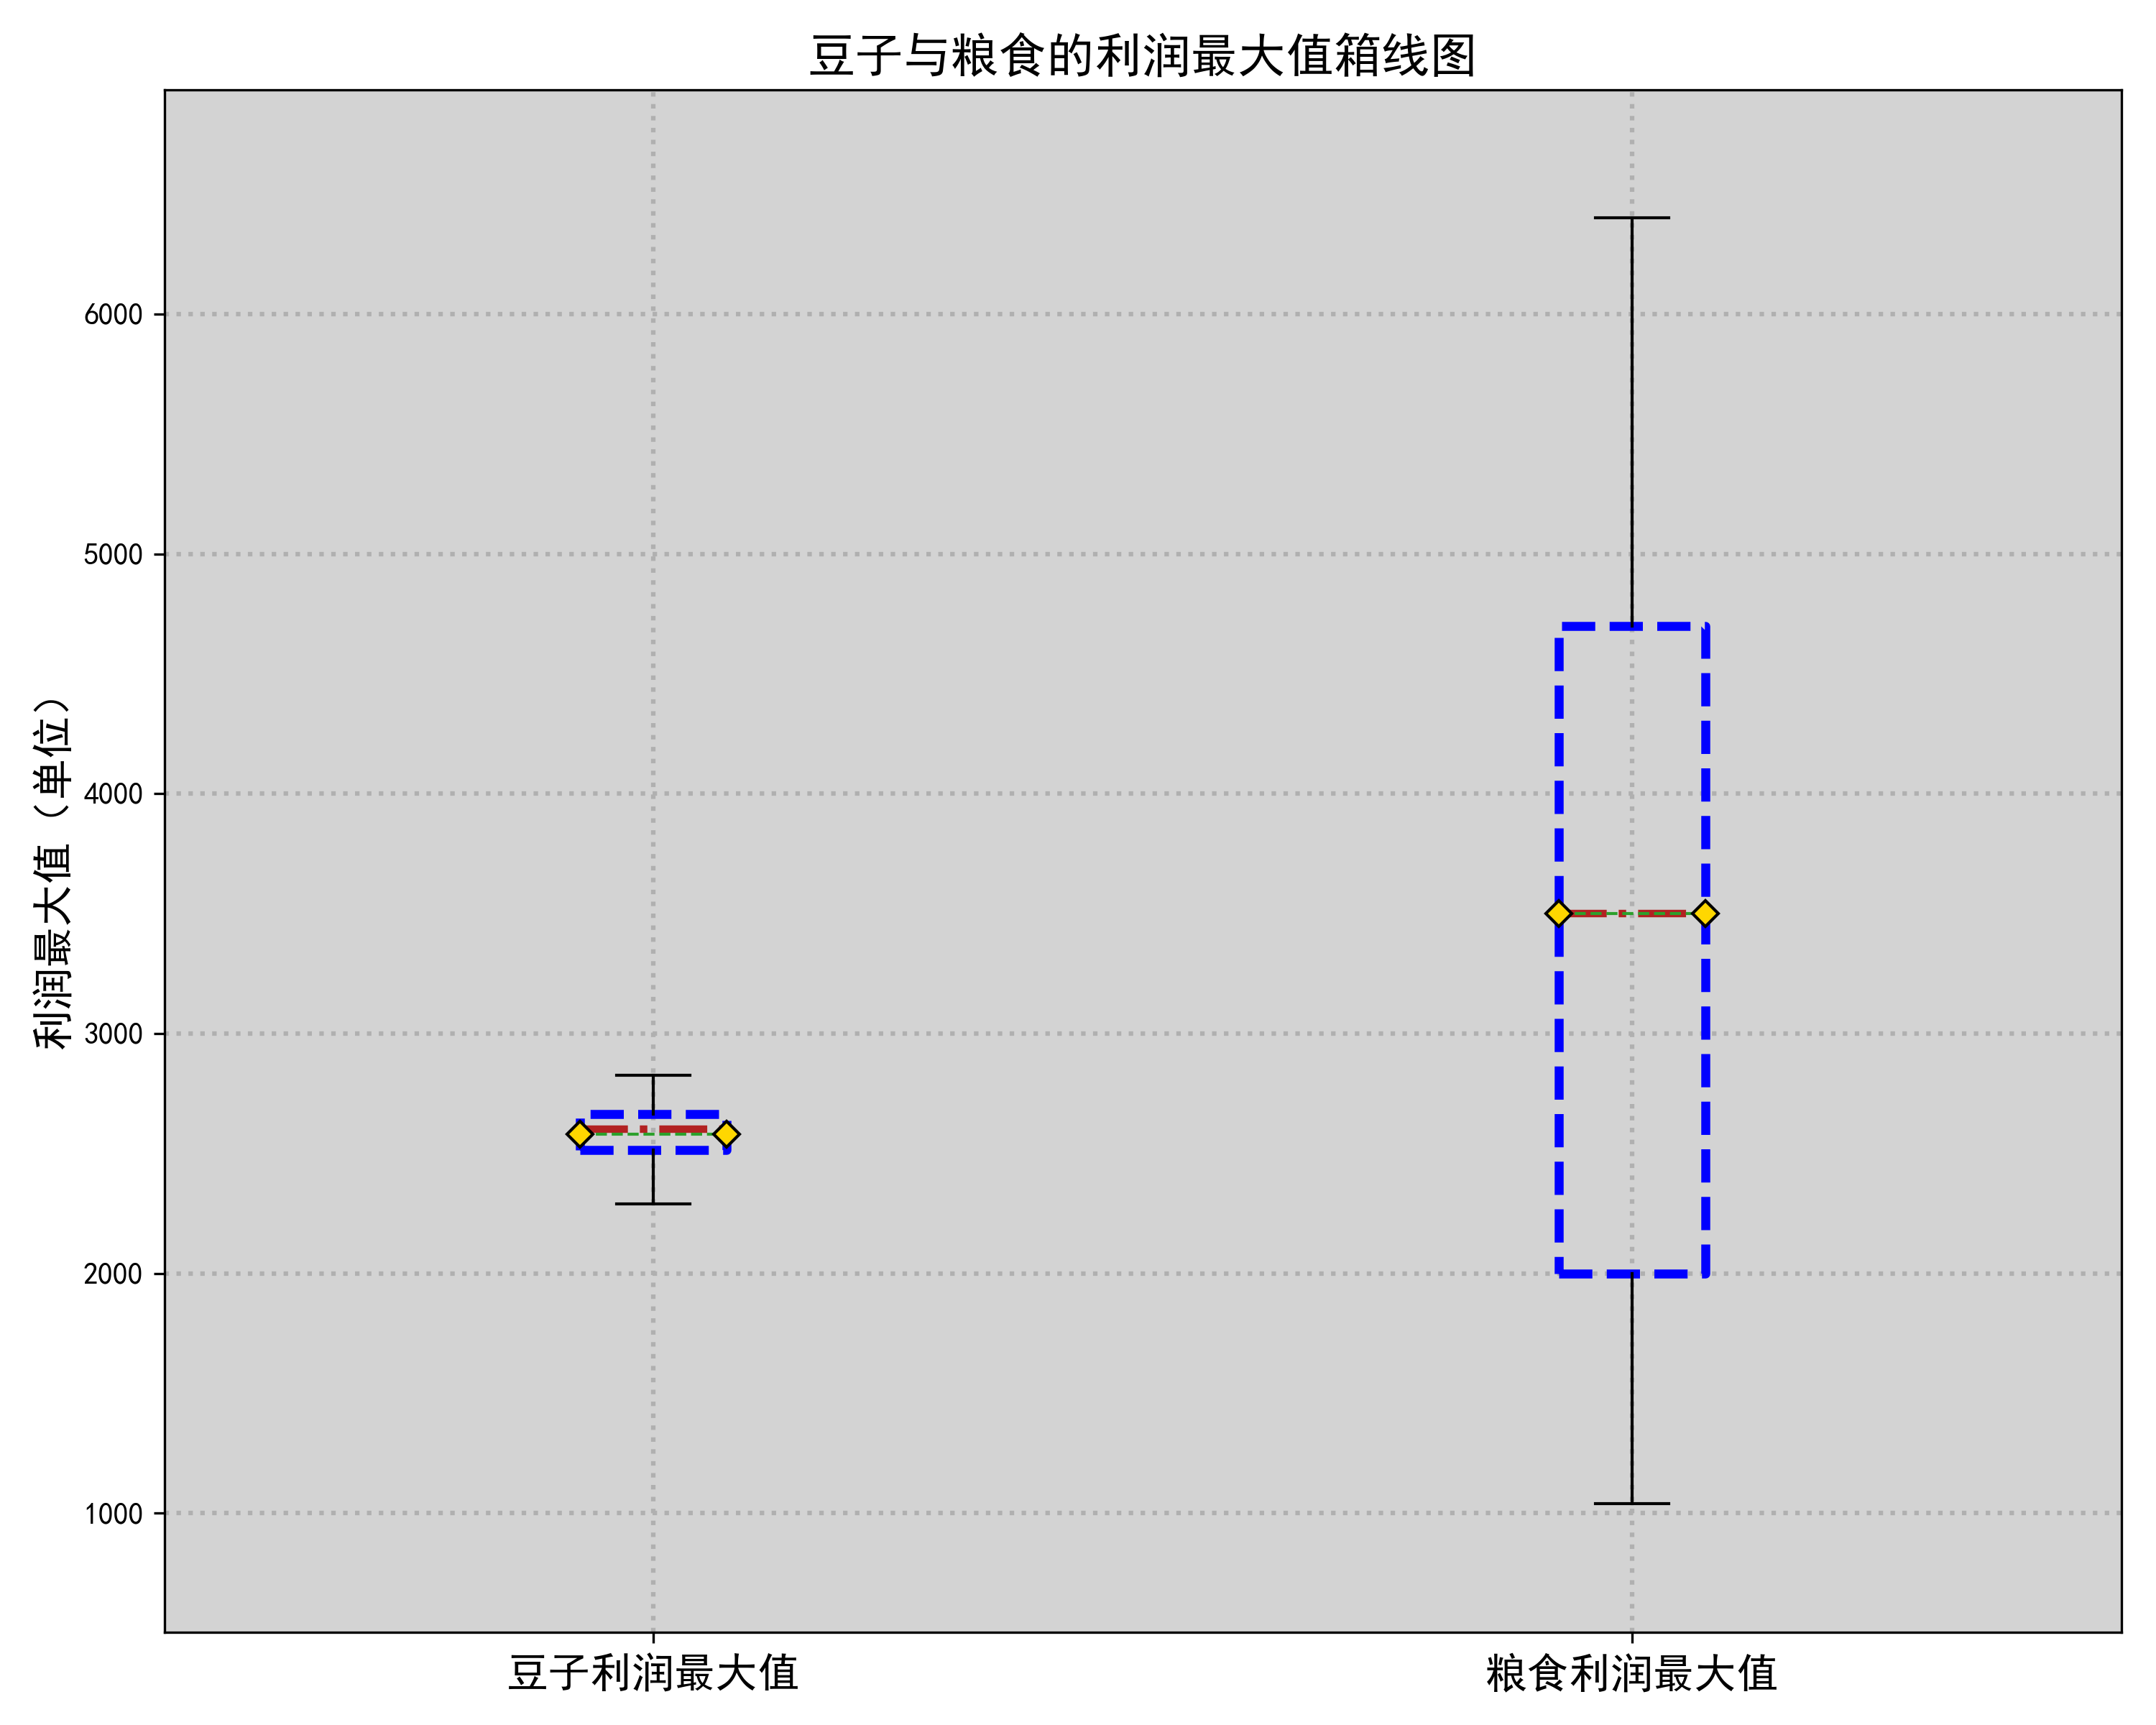
\includegraphics[width=\linewidth]{image7.png}
			\caption{豆类与粮食收益对比1}
			\label{fig:yield_comparison1}
		\end{minipage}\hfill
		\begin{minipage}{0.48\textwidth}
			\centering
			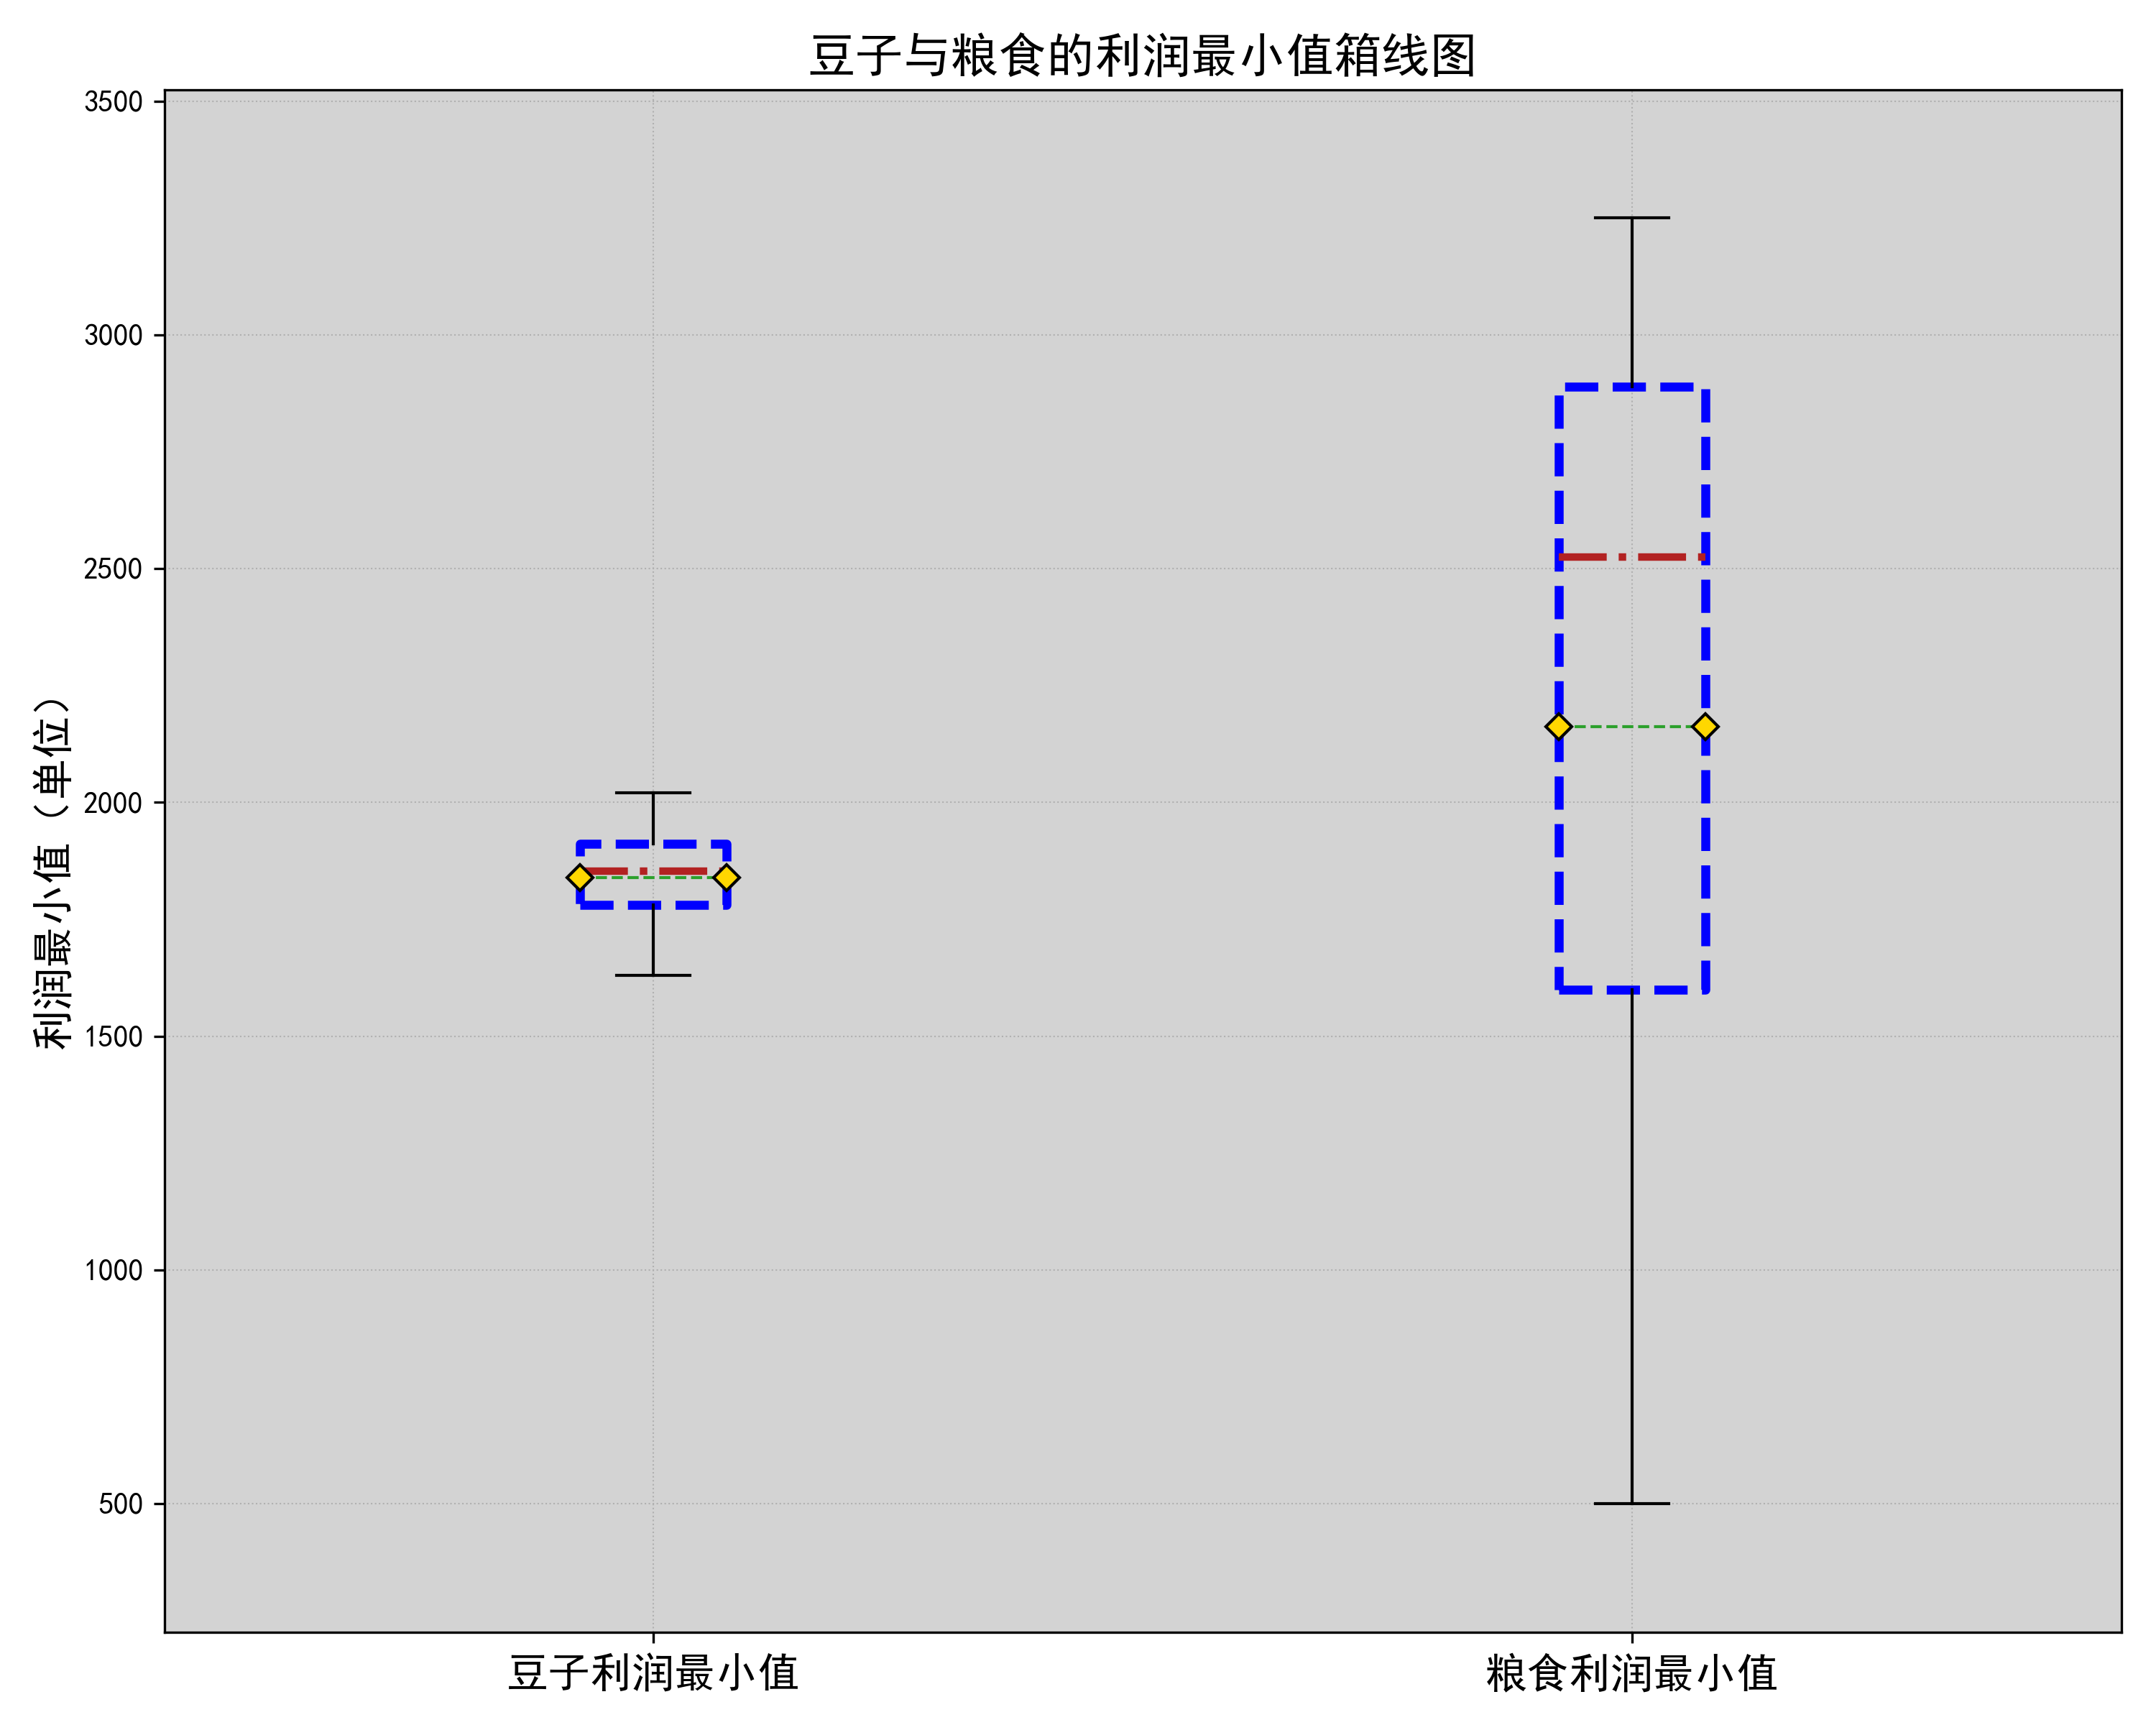
\includegraphics[width=\linewidth]{image8.png}
			\caption{豆类与粮食收益对比2}
			\label{fig:yield_comparison2}
		\end{minipage}
	\end{figure}
	
	
\begin{figure}[h]
	\centering
	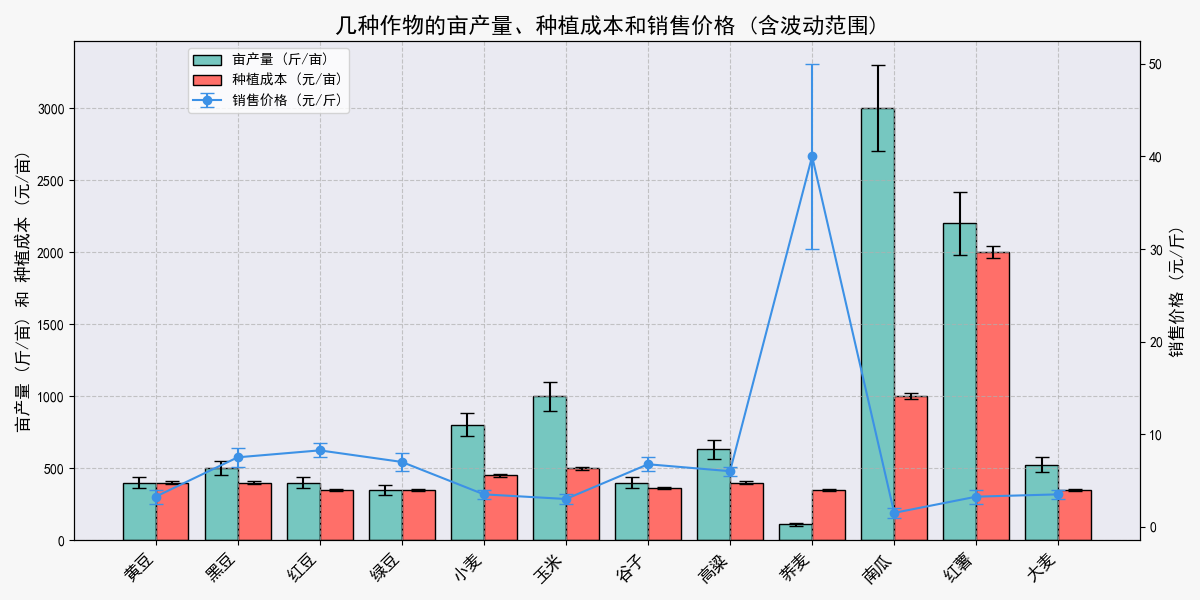
\includegraphics[width=0.8\textwidth]{image13.png}  % 将宽度增加至 80% 的页面宽度
	\caption{作物指标}
	\label{fig:yield_comparison1}
\end{figure}

\begin{figure}[h]
	\centering
	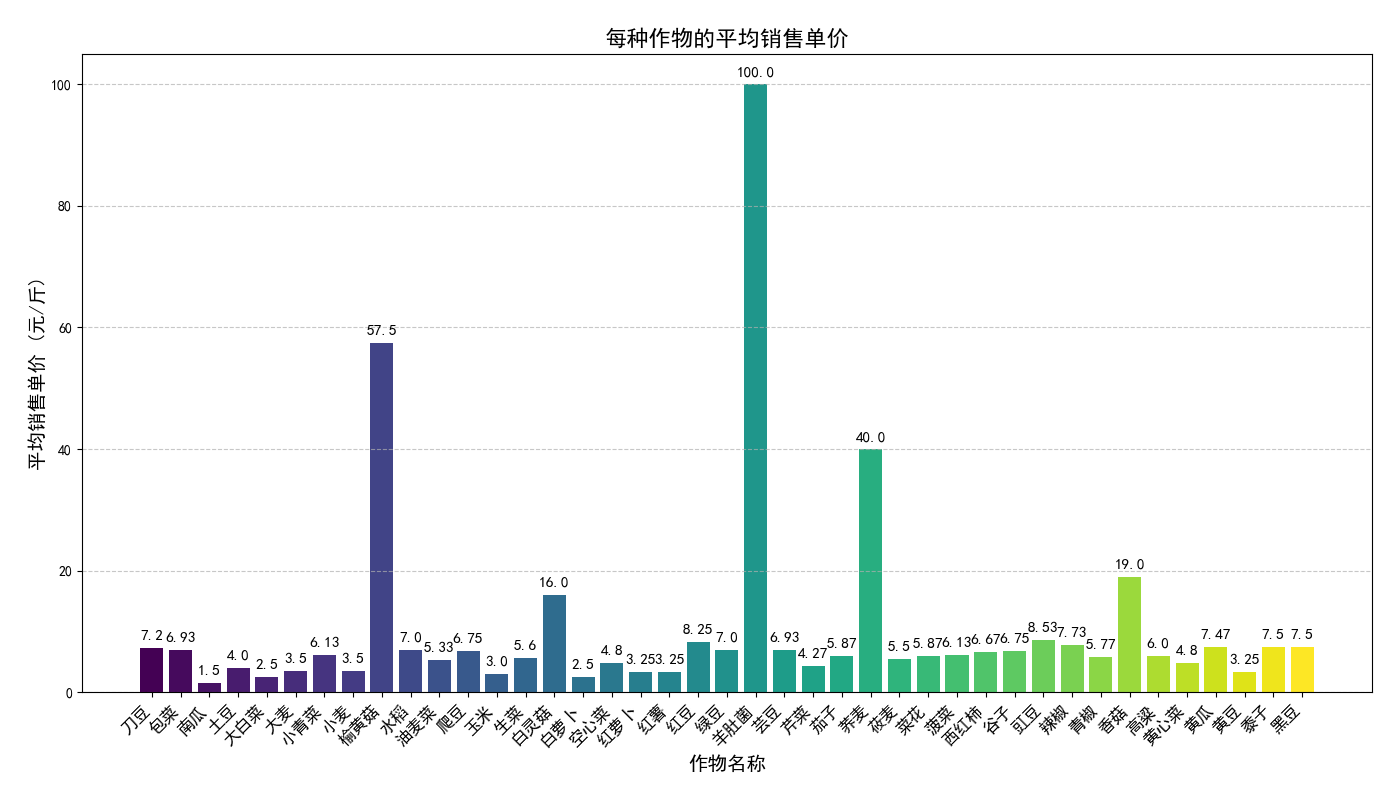
\includegraphics[width=0.8\textwidth]{image14.png}  % 同样将第二张图片调整到 80%
	\caption{作物平均销售单价}
	\label{fig:yield_comparison2}
\end{figure}





	通过箱线图我们可以很明显的看出种植豆类作物的收益均值与中位数均低于种植其他作物,因此假设成立,即应在满足题目约束条件的前提下尽可能少种植豆类作物.

	
	
	首先, 我们在题目给定的的作物售价范围内随机生成价格序列, 记作
 	%不编号
 	\begin{equation*}\vec{y}=\left(y_1, y_2, y_3, \ldots, y_n\right)
	\end{equation*}
	
	\begin{equation} %编号
		\vec{y} =
		\begin{bmatrix}
			y_1 \ y_2 \ y_3 \ldots y_n\\
			y_1 \ y_2 \ y_3 \ldots y_n\\
			y_1 \ y_2 \ y_3 \ldots y_n\\
			\vdots \\
			y_1 \ y_2 \ y_3 \ldots y_n\\
		\end{bmatrix}
		\label{列向量公式}
	\end{equation}
	
	
	其次, 我们使用对数收益正态分布模型生成同等数量的服从正态分布的随机价格序列, 记作
	\begin{equation*}
		\vec{Y}=\left(Y_1, Y_2, Y_3, \ldots, Y_n\right)
	\end{equation*}
	, 计算得残差向量 $\vec{y}-\vec{Y}=\vec{e}=\left(e_1, e_2, e_3, \ldots, e_n\right)$ 。接下来本文进行残差的
	正态性检验并绘制残差 Q-Q 图:
	由图可知样本标准差与标准正态分布标准差比值为拟合直线的斜率, 得到的曲线越接近直线,说明越近似服从正态分布, 斜率越接近 1 说明越近似服从标准正态分布;拟合直线截距表示样本均值。
	对于拟合曲线的尾部行为有以下分析:
	若拟合曲线的尾部二阶导数大于零, 说明模拟变量具有正离群性, 存在比正态分布更多的极端值:
	
	\begin{equation}
	\frac{\sum_{i=1}^n 1 \cdot\left(\left|Y_i-\hat{\mu}\right|>3 \cdot \sigma\right)}{n}>\int_{\left|X_i-\hat{\mu}\right|>3 \cdot \sigma}^{\infty} \frac{1}{\sqrt{2 \cdot \pi \cdot \sigma^2}} \cdot e^{-\frac{(x-\mu)^2}{2 \cdot \sigma^2}} d x
	\end{equation}
	
	若拟合曲线的尾部二阶导数小于零, 说明模型变量具有负离群性, 样体中极端值小于正态分布的极端值:
	
	\begin{equation}
	\frac{\sum_{i=1}^n 1 \cdot\left(\left|Y_i-\hat{\mu}\right|>3 \cdot \sigma\right)}{n}<\int_{\left|X_i-\hat{\mu}\right|>3 \cdot \sigma}^{\infty} \frac{1}{\sqrt{2 \cdot \pi \cdot \sigma^2}} \cdot e^{-\frac{(x-\mu)^2}{2 \cdot \sigma^2}} d x
\end{equation}
	
	
	由本题的残差 $\mathrm{Q}-\mathrm{Q}$ 图可知,拟合曲线尾部特征呈现负离群值, 说明价格分布不仅服从正态分布, 并且离群值更少, 波动范围稳定, 由此即可证实模型假设 2 的正确性。
\end{enumerate}
\begin{figure}[h]
	\centering
	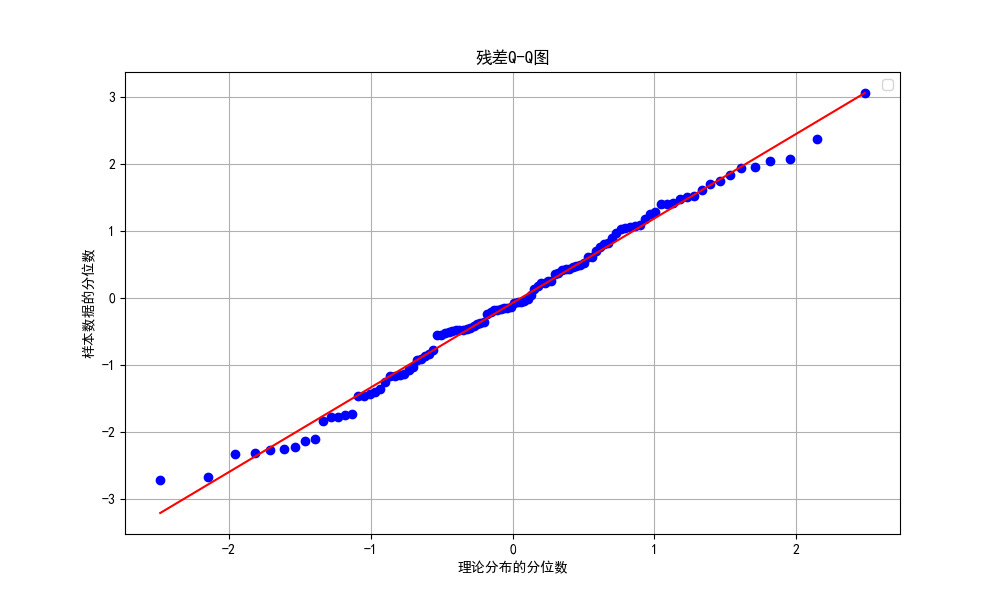
\includegraphics[width=0.9\textwidth]{image15.png}  % 将宽度增加至 80% 的页面宽度
	\caption{残差Q-Q散点拟合}
	\label{fig:yield_comparison1}
\end{figure}

	\section{符号说明}  
	\label{sec:notation}  
	\centering  
	\begin{tabular}{c c}  
		\toprule  
		符号 & 符号含义\\  
		\midrule  
		$S_{i}$ & 第$i$种作物的种植面积/亩\\  
		$P_{i}(t)$ & 第$i$种作物在第$t$年的市场价格/元每斤\\  
		$P_i(T)$ & 第种作物在第年的市场价格(是一个随机变量,受到气候和需求波动的影响\\
		$Q_i(t)$ & 表示第$i$种作物在第年的培育成本/元\\
		$M_i^{(t)}$ & 表示第$i$种作物在第年的市场需求量/斤\\
		$A$ & 总共可种植面积/平方米\\
		$E\left[P_i(t)\right]$ & 农作物$i$在第$t$年的价格期望值/元\\
		$\mu_i$ & 第$i$种作物的价格增长率\\
		$\sigma_i$ & 第$i$种作物的价格波动率,代表价格波动幅度\\
		$d W_t$ & 标准布朗运动(也称之为正态分布随机变量),用于模拟价格波动\\
		$T$ & 未来的时间跨度/年(从2024年开始至2030年,$T=7$)\\
		$N$ & 模拟时间的步数/年\\
		$d t$ & 每个时间步的长度/年\\
		$R(T)$ & $2024-2030$作物的总收益/元\\
		$R_i(T)$ & 作物$i$在$2024-2030$的收益/元\\
		$G$ & 粮食作物的集合\\
		$R$ & 水稻的集合\\
		$m$ & 食用菌的集合\\
		$V$ & 蔬菜的集合\\
		$B$ & 豆类的集合\\
		$m$ & 地块数量\\
		$n$ & 农作物种类数量\\
		\bottomrule  
	\end{tabular}  
	
	\raggedright
	
	\section{问题一求解}  
	\label{sec:solution1}  
	   本题需要根据两个滞销产品处置方法分别设计算法求解最优种植策略,属于单目标多约束的混合整数线性规划。已知预期销售量、种植成本、亩产量和销售价格相较于2023年持平,我们给出以下实现步骤:
	   
	\subsection{定义目标函数}
	\begin{equation}  
		\begin{aligned}  
			& \max R(T) = \sum_{t=2024}^{2030} \sum_{i=1}^n \left[ M_i^{(2023)} \cdot S_i + \left( \delta \cdot P_i(2023) - Q_i(2023) \right) \cdot S_i \right] \\  
			& \text{s.t.} \quad  
			\begin{cases}  
				\delta = 0, & \text{如果超过部分滞销,造成浪费} \\  
				\delta = 0.5, & \text{如果超过部分按2023年销售价50\%降价出售}  
			\end{cases}  
		\end{aligned}  
	\end{equation}  
	
	
	\subsection{条件约束}
	\subsubsection{种植面积总和约束}
	\begin{equation}
		\sum_{i=1}^N S_i \leq A
	\end{equation}

	\subsubsection{非负性约束}
	\begin{equation}\forall i, \quad S_i \geq 0\end{equation}
	
	\subsubsection{地块类型与用途约束}
	\setlength{\parindent}{2em}
	设 $x_{i, j}^{(t)}$ 为地块 j 在第 t 年种植第 i 种作物的二进制决策变量
	
	(1)露天耕地只能种植一季的粮食类作物设 $L_1$ 为露天耕地的地块索引集合,则对于每个 $j \in L_1$ ,有:
	
	\begin{equation}
	\forall j \in L_1, \quad \forall t, \quad \sum_{i \in G} x_{i, j}^{(t)} \leq 1
	\end{equation}
	
	(2)水浇地可以种植一季水稻或两季蔬菜设 $L_2$ 为水浇地的地块索引集合, 则对于每个 $j \in L_2$, 每年要么种一季水稻, 要么种两季蔬菜:
	
	\begin{equation}
	\forall j \in L_2, \quad \forall t, \quad \sum_{i \in R} x_{i, j}^{(t)}+\sum_{i \in V} x_{i, j}^{(t)} \leq 2
	\end{equation}
	
	
	(3)普通大棚只能种一季的蔬菜或一季的食用菌设 $L_3$ 为普通大棚地块索引的集合, 则对于每个 $j \in L_3$, 每年只能种植一季的蔬菜或一季的食用菌:
	
	\begin{equation}
	\forall j \in L_3, \quad \forall t, \quad \sum_{i \in V U M} x_{i, j}^{(t)} \leq 1
	\end{equation}
	
	(4)智慧大棚只能种两季的蔬菜设 $L_4$ 为智慧大棚的地块索引集合, 每年只能种两季蔬菜:
	
	\begin{equation}
	\forall j \in L_4, \quad \forall t, \quad \sum_{i \in V} x_{i, j}^{(t)}=2
	\end{equation}
	
	
	(3) 普通大棚只能种一季的蔬菜或一季的食用菌设 $L_3$ 为普通大棚地块索引的集合, 则对于每个 $j \in L_3$, 每年只能种植一季的蔬菜或一季的食用菌:
	
	\begin{equation}
	\forall j \in L_3, \quad \forall t, \quad \sum_{i \in V U M} x_{i, j}^{(t)} \leq 1
	\end{equation}
	
	(4)智慧大棚只能种两季的蔬菜
	设 $L_4$ 为智慧大棚的地块索引集合, 每年只能种两季蔬菜:
	
	\begin{equation}
	\forall j \in L_4, \quad \forall t, \quad \sum_{i \in V} x_{i, j}^{(t)}=2
	\end{equation}
\subsubsection{可持续性发展约束}
	(1)同一种类型地块不能连续重茬种植
	作物 $i$ 在地块 $j$ 上的种植不能连续发生在相邻的两年中:
	
	\begin{equation}
	\forall j \in L_{\varepsilon}(\varepsilon \in\{1,2,3,4\}), \quad \forall t, \quad \sum_{i \in X} x_{i, j}^{(t)}+\sum_{i \in X} x_{i, j}^{(t+1)} \leq 1
	\end{equation}
	
	$X$ 为单元素集合,且 $X \subseteq\{G, R, V, M\}$
	(2) 同种类型地块 3 年内不能没有豆类种植
	
	由已验证的假设知, 豆类作物经济效益极低, 故每连续三年内只有
	一年种植豆类作物:
	
	\begin{equation}
	\forall j \in L_{\varepsilon}(\varepsilon \in\{1,2,3,4\}), \quad \forall t, \quad \sum_{i \in B} x_{i, j}^{(t)}+\sum_{i \in B} x_{i, j}^{(t+1)}+\sum_{i \in B} x_{i, j}^{(t+2)}=1
	\end{equation}
	并且2024-2030年之间有两年种植豆类植物
	\begin{table}[htbp]
	\centering
	\begin{tabular}{|c|c|c|c|c|c|c|c|c|}
		\hline  
		年份 & 2023 & 2024 & 2025 & 2026 & 2027 & 2028 & 2029 & 2030 \\
		\hline
		方案 1 & 1 & 0 & 0 & 1 & 0 & 0 & 1 & 0 \\
		\hline
		方案 2 & 1 & 0 & 0 & 1 & 0 & 1 & 0 & 0 \\
		\hline
		方案 3 & 1 & 0 & 1 & 0 & 0 & 1 & 0 & 0 \\
		\hline
		方案 4 & 0 & 0 & 1 & 0 & 0 & 1 & 0 & 0 \\
		\hline
	\end{tabular}  
	\caption{不同年份的不同方案分析}
\end{table}
	\subsubsection{风险控制约束}
	
	使用在险价值 $(V a R)$ 度量工具进行风险限制, 在 $\alpha=95 \%$ 的置信水平下,设最低收益为 $R_0$, 则要求:
	
	\begin{equation}
	P\left(R_i(T)>R_0\right) \geq \alpha
	\end{equation}
	
	\begin{figure}[h]
		\centering
		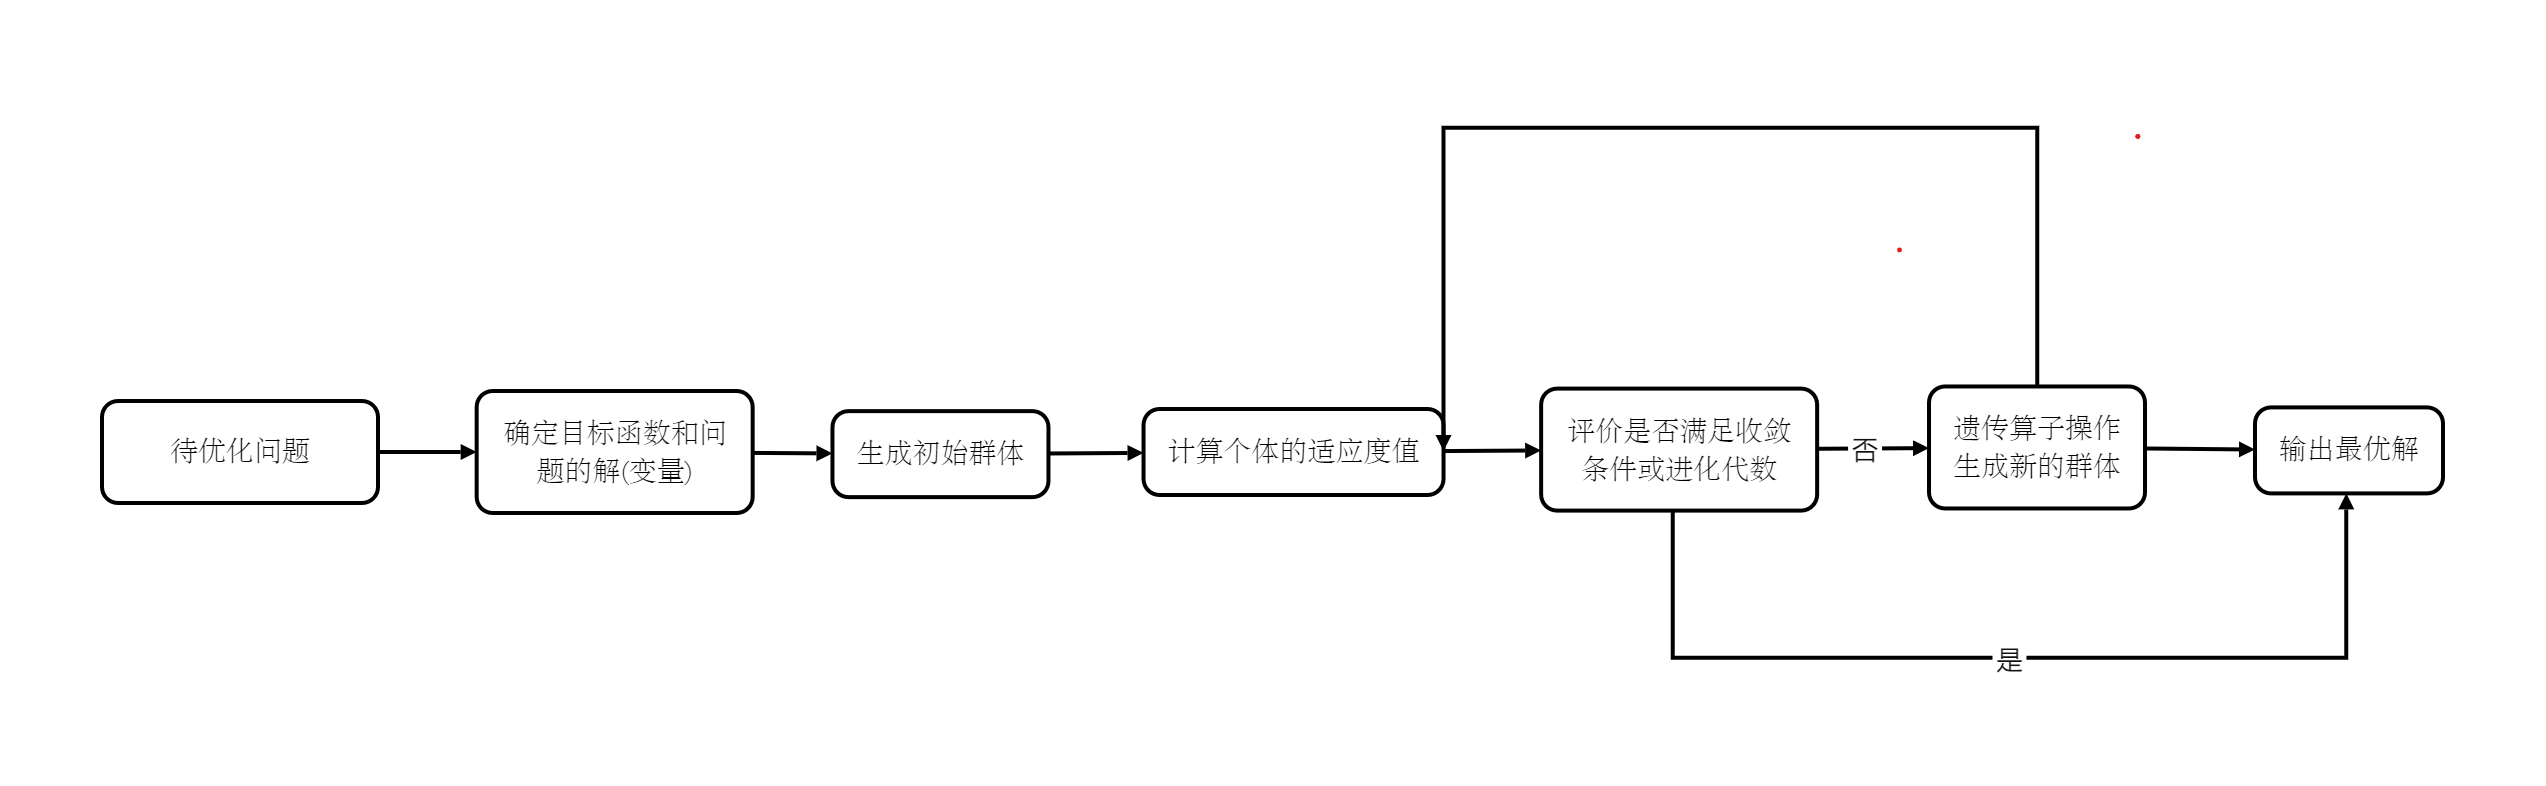
\includegraphics[width=0.8\textwidth]{image19.png}  % 将宽度增加至 80% 的页面宽度
		\caption{遗传算法流程图}
		\label{fig:yield_comparison1}
	\end{figure}
	\subsection{遗传算法模型求解}
	\subsubsection{参数输入}
	基因初始化:每个基因随机取值 0, 0.5, 1 个体初始化:令个体 $\vec{x} \in \mathbb{R}^n, n$ 表示维数
	\subsubsection{种群生成}
	随机生成 m 个个体, 每个个体都是 n 维向量, 种群即:
	\begin{equation}
		\text{m} \times \text{n} \text{ 矩阵 } P = \left(\overrightarrow{x_1}, \overrightarrow{x_2}, \overrightarrow{x_3}, \ldots, \overrightarrow{x_m}\right)
	\end{equation}
	\subsubsection{适应度函数}
	目标是最大化利润 $R(T)$, 适应度函数为:
	
	\begin{equation}
	R(T)=\sum_{i=1}^n \operatorname{Profit}\left(\overrightarrow{x_i}\right)
\end{equation}
	
	$\operatorname{Profit}\left(\vec{x}_i\right)$ 是第 i 个基因对应的收益
	\subsubsection{交叉操作}
	本题使用两点交叉策略, 可描述为:
	
	\begin{equation}
	\overrightarrow{x_{\text {child }}}=\overrightarrow{x_{\text {parent } 1}^{\left[0: c_1\right]}}+\overrightarrow{x_{\text {parent } 2}^{\left[c_1: c_2\right]}}+\overrightarrow{x_{\text {parent } 1}^{\left[c_2: 0\right]}}
\end{equation}
	
	$c_1, c_2$ 是交叉点
	\subsubsection{变异操作}
	选择基于概率 p 的基因位翻转操作, 变异可描述为:
	
\begin{equation}
	\overrightarrow{x_{\text {new }}^{[i]}}=\left\{\begin{array}{cc}
		1-\overline{x^{[i]}} & \text { 概率为 } p \\
		\overline{x^{[i]}} & \text { 概率为 } 1-p
	\end{array}\right.
\end{equation}
	
	
	P取 0.05
	\subsubsection{选择操作}
	从当前种群中使用锦标赛选择法选择个体用于交又和变异:
	$\operatorname{Select}(t)=\operatorname{argmax}\left(\left\{R_i(T) \mid \overrightarrow{x_i} \in\right.\right.$ Tournament $\left.\}\right)$
	Tournament是从种群中随机选择个体的 3 元素集合
	\subsubsection{最优解图示}

\begin{figure}[h]
\centering
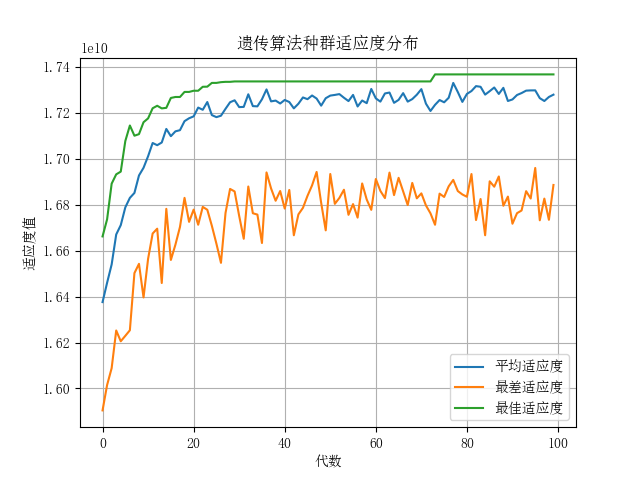
\includegraphics[width=0.9\textwidth]{image21.png}  % 将宽度增加至 80% 的页面宽度
\caption{最优解的种群分布}
\label{fig:yield_comparison1}
\end{figure}
	
	
	
	
	
	
	
	
	
	
	\section{问题二求解}  
	\label{sec:solution2}  
	第二题的要求根据不同作物的种植面积、气候、市场需求及价格波动的影响,建立一个概率规划模型来优化2023年至2030年间的种植策略。考虑到市场价格的和需求的波动,该问题需要给出价格,需求量等变量的关于时间的函数以及波动的概率分布,我们采用概率规划模型,结合农作物种植策略优化,给出以下实现步骤:
	\subsection{定义目标函数}
	目标是最大化从 2024 年到 2030年的总期望收益。基于作物的价格 $P_i(t)$
	在一定范围的波动的假设, 种植收益可以用期望形式表示:
	
	\begin{equation}
	R(T)=\max E\left[\sum_{t=2024}^{2030} \sum_{i=1}^n \min \left(\left(P_i(t)-Q_i(t)\right) \cdot S_i\left(P_i(t)-Q_i(t)\right) \cdot M_i^{(t)}\right)\right]
	\end{equation}
	
	\subsection{构造价格的概率分布模型}
	根据问题描述,基于每年作物价格的波动范围内作物价格的取值服从正态分布的假设,建立基于几何布朗运动(GBM)的对数收益正态分布模型,对价格的波动进行模拟,过程如下:
	\subsubsection{GBM描述价格随时间变化的随机过程的微分方程形式}
	
	\begin{equation}
	d P_i(t)=\mu_i \cdot P_i(t) d t+\sigma_i \cdot P_i(t) d W_t
	\end{equation}
	
	
	公式含义:
	
	价格变化由两部分组成:
	
	确定性部分:与价格成正比的增长, 反映了长期平均趋势
	\begin{equation*}\mu_i \cdot P_i(t) d t\end{equation*} 
	
	
	随机性部分:与价格成正比的随机波动,反映了短期波动
	\begin{equation*}\sigma_i \cdot P_i(t) d W_t:\end{equation*} 
	
	\subsubsection{对数收益形式}
	通过积分可以得到价格的显式解(从初始价格 $P_i(0)$ 开始):
	
	\begin{equation}
	P_i(t)=P_i(0) \cdot \exp \left(\left(\mu_i-\frac{\sigma_i^2}{2}\right) \cdot t+\sigma_i \cdot W_t\right)
	\end{equation}
	
	
	取自然对数, 得到作物价格的对数形式:
	
	\begin{equation}
	\ln P_i(t)=\ln P_i(0)+\left(\mu_i-\frac{\sigma_i^2}{2}\right) \cdot t+\sigma_i \cdot W_t
\end{equation}
	
	
	即作物的对数价格在时间 t 内服从正态分布:
	
	\begin{equation}
	\ln P_i(t) \backsim N\left(\mu_i, \sigma_i^2\right)
\end{equation}
	\subsubsection{模拟收益生成路径}  
	\begin{enumerate}  
		\item 输入参数:  
		\begin{itemize}  
			\item $P_i(0)$:初始价格取销售价格范围内最大值与最小值的均值  
			\item $T = 7$:时间跨度(年)  
			\item $N = 1000$:模拟样本数量  
		\end{itemize}  
	\end{enumerate}
	
	算法步骤:
	\newline
	
	
	\textbf{1.初始化:}令 \[d t=\frac{T}{N}\]
	
	
	\textbf{2.循环生成每个时间步的价格:}

	对 $j=1,2, \ldots N$ (每个时间步), 生成价格轨迹:
	随机生成一个标准正态分布随机数
	\begin{equation}
	Z_j \sim N(0,1)
	\end{equation}
	
	
	计算每一个时间步的对数收益
	\begin{equation}
	\ln P_i\left(t_j\right)=\ln P_i\left(t_{j-1}\right)+\left(\mu_i-\frac{\sigma_i^2}{2}\right) d t+\sigma_i \sqrt{d t} \cdot Z_j
	\end{equation}
	
	
	恢复到价格空间
	\begin{equation}
	\begin{aligned}
		& P_i\left(t_j\right)=\exp \left(\ln P_i\left(t_j\right)\right) \\
		& t_j=j \cdot d t
	\end{aligned}
    \end{equation}
    
    
	\textbf{3. 重复模拟:}
	重复上述过程 1000 次, 获得足量作物价格的不同可能路径, 用于统计分析
	
	
	\textbf{4.求期望与风险度量:}

	对于每一条路径,计算其对应的收益:
	\begin{equation}
	\ln P_i\left(t_j\right)=\ln P_i\left(t_{j-1}\right)+\left(\mu_i-\frac{\sigma_i^2}{2}\right) d t+\sigma_i \sqrt{d t} \cdot Z_j
	\end{equation}
	
	
	求对应的价格期望:
	
	\begin{equation}
	P_i\left(t_j\right)=\exp \left(\ln P_i\left(t_j\right)\right)
	\end{equation}
	
	
	\subsubsection{计算风险度量:}
	
	
	\textbf{(1)生成价格路径}
	
	从初始时间 $t_0$ 开始, 生成 $M$ 条农作物价格的未来路径 $P_i(t)$,
	每条路径包含多个时间步
	对于每条路径,在目标时间节点得到最终价格
	
	
		\textbf{(2)计算收益}
	
	对于每一条价格路径, 我们可以得到一个对应的总收益值
	
		\begin{equation}
	R_i(T)=S_i \cdot\left(P_i(t)-Q_i(t)\right)
	\end{equation}


	\textbf{(3)计算收益的分布}
	
	通过模拟 $M$ 条不同的价格路径, 我们可以得到一个对应的总收益值分布序列:
	
		\begin{equation}
	\overrightarrow{R_i}=\left\{R_i(1), R_i(2), R_i(3), \ldots, R_i(N)\right\}
\end{equation}
	
	
	该序列存储了每条价格路径在时间跨度 $T$ 内的总收益
	
	
	\textbf{(4) 计算在险价值 $($ VaR $)$}
	\[V a R\]
	
	
	表示在某一置信水平下可能出现的最大损失
	
	
	算法步骤如下:
	
	
	(1) 设定置信水平 $\alpha=95 \%$, 即本模型有 $95 \%$ 的把握使损失不超过某个特定值
	
	
	(2)对收益序列排升序,得到排序后的收益序列
	
	
	\begin{equation}
	\overrightarrow{R_{\text {sorted }}}=\left\{R_i^*(1), R_i^*(2), R_i^*(3), \ldots, R_i^*(N)\right\}
\end{equation}


	(3)计算 $V a R_\alpha$ : 在 $1-\alpha=5 \%$ 的置信水平下, $V a R$ 是这个序列中第 $(1-\alpha) \cdot M$ 个收益值。计算公式:
		\begin{equation}
	\operatorname{VaR}_\alpha=\text { percentile } 1-\alpha\left(R_i\right)
\end{equation}


	同理可对销量,成本进行预测
	
	\subsection{条件约束}
	\subsubsection{种植面积总和约束:}
	
	\begin{equation}
	\sum_{i=1}^N S_i \leq A
\end{equation}
	
	\subsubsection{非负性约束:}
	\[
	\forall i ,\quad S_i \geq 0
	\]
	
\subsubsection{地块类型与用途约束:}
	
	设 $x_{i, j}^{(t)}$ 为地块 j 在第 t 年种植第 i 种作物的二进制决策变量
	
	
	①:露天耕地只能种植一季的粮食类作物
	
	设 $L_1$ 为露天耕地的地块索引集合
	则对于每个 $j \in L_1$ ,有:
	
	\begin{equation}
	\forall j \in L_1, \quad \forall t, \quad \sum_{i \in G} x_{i, j}^{(t)} \leq 1
\end{equation}
	
	②:水浇地可以种植一季水稻或两季蔬菜
	
	设 $L_2$ 为水浇地的地块索引集合, 则对于每个 $j \in L_2$, 每年要么种一季水稻,要么种两季蔬菜:
	
	\begin{equation}
	\forall j \in L_2, \quad \forall t, \quad \sum_{i \in R} x_{i, j}^{(t)}+\sum_{i \in V} x_{i, j}^{(t)} \leq 2
\end{equation}
	
	③:普通大棚只能种一季的蔬菜或一季的食用菌
	
	设 $L_3$ 为普通大棚地块索引的集合,
	则对于每个 $j \in L_3$ ,每年只能种植一季的蔬菜或一季的食用菌:
	
	\begin{equation}
	\forall j \in L_3, \quad \forall t, \quad \sum_{i \in V \cup M} x_{i, j}^{(t)} \leq 1
\end{equation}
	
	④:智慧大棚只能种两季的蔬菜
	
	设 $L_4$ 为智慧大棚的地块索引集合,每年只能种两季蔬菜:
	
		\begin{equation}
	\forall j \in L_4, \quad \forall t, \quad \sum_{i \in V} x_{i, j}^{(t)}=2
\end{equation}
	
	\subsubsection{可持续性发展约束:}
	同一种类型地块不能连续重茬种植
	
	作物 $i$ 在地块 $j$ 上的种植不能连续发生在相邻的两年中:
	\begin{equation}
	\forall j \in L_{\varepsilon}(\varepsilon \in\{1,2,3,4\}), \quad \forall t, \quad \sum_{i \in X} x_{i, j}^{(t)}+\sum_{i \in X} x_{i, j}^{(t+1)} \leq 1
    \end{equation}
	
	$X$ 为单元素集合, 且 $X \subseteq\{G, R, V, M\}$
	6.3.4.2 同种类型地块 3 年内不能没有豆类种植
	
	由已验证的假设知, 豆类作物经济效益极低, 故每连续三年内只有一年种植豆类作物:
	\begin{equation}
	\forall j \in L_{\varepsilon}(\varepsilon \in\{1,2,3,4\}), \forall t, \quad \sum_{i \in B} x_{i, j}^{(t)}+\sum_{i \in B} x_{i j}^{(t+1)}+\sum_{i \in B} x_{i, j}^{(t+2)}=1
\end{equation}
	
	
	并且 2024-2030 年之间有两年种植豆类植物
	\begin{table}[htbp]
		\centering
		\begin{tabular}{|c|c|c|c|c|c|c|c|c|}
			\hline  
			年份 & 2023 & 2024 & 2025 & 2026 & 2027 & 2028 & 2029 & 2030 \\
			\hline
			方案 1 & 1 & 0 & 0 & 1 & 0 & 0 & 1 & 0 \\
			\hline
			方案 2 & 1 & 0 & 0 & 1 & 0 & 1 & 0 & 0 \\
			\hline
			方案 3 & 1 & 0 & 1 & 0 & 0 & 1 & 0 & 0 \\
			\hline
			方案 4 & 0 & 0 & 1 & 0 & 0 & 1 & 0 & 0 \\
			\hline
		\end{tabular}  
		\caption{不同年份的方案分析}
	\end{table}
	
	使用在险价值 $(V a R)$ 度量工具进行风险限制,在 $\alpha=95 \%$ 的置信水平下,设最低收益为 $R_0$, 则要求:
	\begin{equation}
	P\left(R_i(T)>R_0\right) \geq \alpha
\end{equation}
	
	\subsection{鲁棒优化模型求解}
		\begin{figure}[h]
		\centering
		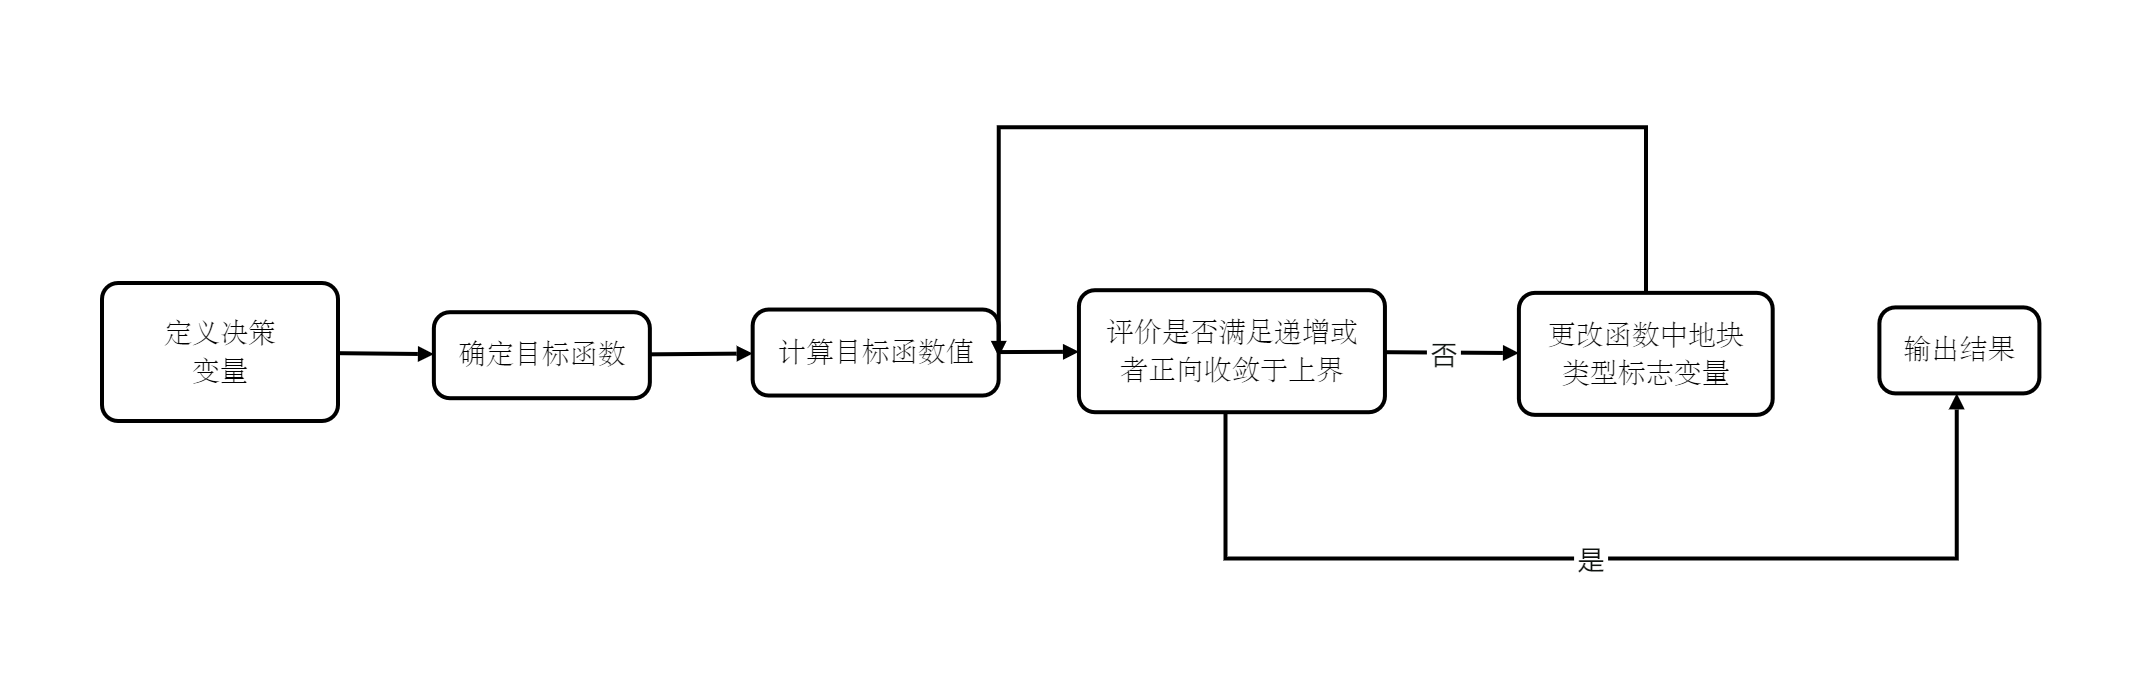
\includegraphics[width=0.8\textwidth]{image18.png}  % 将宽度增加至 80% 的页面宽度
		\caption{鲁棒优化流程图}
		\label{fig:yield_comparison1}
	\end{figure}
	
	由题意,本题数据存在波动,若继续设计常规的单目标规划模型容易造成较大误差。所以我们使用鲁棒优化算法求解,过程如下:
	\subsubsection{定义决策变量}
设 $X_{i, k, t, j}$为地块$i$在年份$t$的季节$j$是否种植作物$k$
\begin{equation}
\begin{aligned}
	& x_{i, k, t, j}= \begin{cases}0 & \text { 不种植 } \\
		1 & \text { 种植 }\end{cases} \\
	& j= \begin{cases}1 & \text { 第一季 } \\
		2 & \text { 第二季 }\end{cases}
\end{aligned}
\end{equation}

	\subsubsection{确定目标函数}
	\textbf{定义地块类型标志变量 $l_{\text {index }}(i)$}
	
	
\begin{equation}
	\begin{gathered}
		l_{\text{single}}(i) = 
		\begin{cases}
			1 & \text{地块 } i \text{ 是单季地} \\
			0 & \text{地块 } i \text{ 不是单季地}
		\end{cases} \\
		l_{\text{double\_irrigated}}(i) = 
		\begin{cases}
			1 & \text{地块 } i \text{ 是双季水浇地} \\
			0 & \text{地块 } i \text{ 不是双季水浇地}
		\end{cases} \\
		l_{\text{greenhouse}}(i) = 
		\begin{cases}
			1 & \text{地块 } i \text{ 是普通大棚} \\
			0 & \text{地块 } i \text{ 不是普通大棚}
		\end{cases} \\
		l_{\text{smartgreenhouse}}(i) = 
		\begin{cases}
			1 & \text{地块 } i \text{ 是智慧大棚} \\
			0 & \text{地块 } i \text{ 不是智慧大棚}
		\end{cases}
	\end{gathered}
\end{equation}



	\textbf{设置目标参数}
	\begin{equation}
	\max R(T)=\sum_{t=2024}^{2030} \sum_{i=1}^m \sum_{k=1}^n \sum_{j \in[1,2]} l_{\text {index }}(i) \cdot\left[P_i(t)-Q_i(t)\right] \cdot A \cdot X_{i, k, t, j}
\end{equation}
	
	
	
	\subsubsection{输出结果}
 体现在农作物种植决策的结果如下:
\begin{table}[htbp]
	\centering
	\begin{tabular}{m{5cm} m{5cm} m{6cm}}  
		\toprule  
		地块类型 & 年份 & 种植作物及其比例\\  
		\midrule  
		A平旱地 & 偶数年 & 红薯 90\%, 其余 10\%\\  
		B梯田 & 偶数年& 红薯 90\%, 其余 10\%\\  
		C山坡地  & 偶数年&  红薯 90\%, 其余 10\%\\
		D 水浇地 & 偶数年第一季 & 茄子 100\% \\
		D 水浇地 & 偶数年第二季 & 水稻 100\% \\
		E 普通大棚 & 第一季 & 豇豆 90\%, 刀豆 10\% \\
		E 普通大棚 & 第二季 & 豆豆 100\% \\
		F 智慧大棚 & 第一季 & 茄子 60\%, 土豆 20\%, 西红柿20\% \\
		F 智慧大棚 & 第二季 & 豇豆 70\%, 刀豆 30\% \\
		\bottomrule  
	\end{tabular}  
	\caption{种植策略1}
\end{table}
由图可知,单季地从整体收益看无须区分奇数年和偶数年,且一年一季,均安排种植百分之90红薯和百分之10其他成本较低且有利于可持续性发展的作物。水浇地需要安排轮作,奇数年第一季种植百分之30豇豆,百分之70茄子,第二季全部种植水稻,偶数年第一季全部种植茄子,第二季全部种植水稻。


	
	
	\newpage
	\section{问题三求解}  
	\label{sec:solution3}  
	本问题要求我们考虑农作物之间的可替代性和互补性,并根据这种关系为 2024-2030 年设计最优种植方案。通过引入经济学中的交叉弹性,分析作物之间的相互影响,可以优化种植组合,提高总收益并降低亏本风险。以下是利用交叉弹性解决此问题的具体算法步骤:
	\subsection{预期销售量、亩产量和种植成本的相关性分析}
	我们利用python斯皮尔曼相关系数分析,得到结果如图8
	
	
	由图可知,亩产量与种植成本之间具有较强的正相关性;平均销售单价与种植成本之间几乎不存在关联性;此外,平均销售单价与亩产量之间则展现出一种微弱的负相关性,表明在一定程度上,亩产量的提高可能会伴随着平均销售单价的轻微下降。
	\begin{figure}[h]
		\centering
		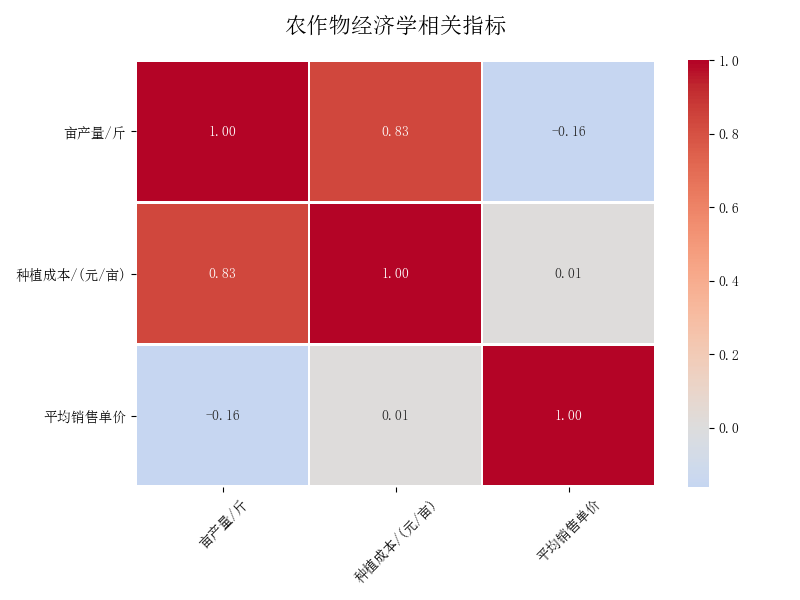
\includegraphics[width=0.8\textwidth]{image20.png}  % 将宽度增加至 80% 的页面宽度
		\caption{作物指标}
		\label{fig:yield_comparison1}
	\end{figure}
	\subsection{建立交叉弹性矩阵}
$E_{x, y}$ 表示作物 $x$ 对作物 $y$ 的需求交叉弹性:
%交叉弹性矩阵 $(5 \times 5)$ 为:
\begin{equation}
	E = \left[
	\begin{array}{lllll}
		E_{G, G} & E_{G, R} & E_{G, V} & E_{G, M} & E_{G, B} \\
		E_{R, G} & E_{R, R} & E_{R, V} & E_{R, M} & E_{R, B} \\
		E_{V, G} & E_{V, R} & E_{V, V} & E_{V, M} & E_{V, B} \\
		E_{M, G} & E_{M, R} & E_{M, V} & E_{M, M} & E_{M, B} \\
		E_{B, G} & E_{B, R} & E_{B, V} & E_{B, M} & E_{B, B}
	\end{array}
	\right]
\end{equation}
	
	\subsection{条件约束}
	\subsubsection{种植面积总和约束}
	
\begin{equation}
	\sum_{i=1}^N S_i \leq A
\end{equation}
	\subsubsection{非负性约束}
	\begin{equation}
	\forall i, \quad S_i \geq 0
\end{equation}
	\subsubsection{地块类型与用途约束}
	
	设 $x_{i, j}^{(t)}$ 为地块 j 在第 t 年种植第 i 种作物的二进制决策变量
	\newline
	(1)露天耕地只能种植一季的粮食类作物
	设 $L_1$ 为露天耕地的地块索引集合, 则对于每个 $j \in L_1$, 有:
	\begin{equation}\forall j \in L_1, \quad \forall t, \quad \sum_{i \in G} x_{i, j}^{(t)} \leq 1\end{equation}
	(2)水浇地可以种植一季水稻或两季蔬菜
	设 $L_2$ 为水浇地的地块索引集合, 则对于每个 $j \in L_2$, 每年要么种一季水稻, 要么种两季蔬菜:
	
\begin{equation}
	\forall j \in L_2, \quad \forall t, \quad \sum_{i \in R} x_{i, j}^{(t)}+\sum_{i \in V} x_{i, j}^{(t)} \leq 2
\end{equation}
	
	(3)普通大棚只能种一季的蔬菜或一季的食用菌设 $L_3$ 为普通大棚地块索引的集合, 则对于每个 $j \in L_3$, 每年只能种植一季的蔬菜或一季的食用菌:
	
\begin{equation}
	\forall j \in L_3, \quad \forall t, \quad \sum_{i \in V U M} x_{i, j}^{(t)} \leq 1
\end{equation}
	
	(4)智慧大棚只能种两季的蔬菜
	设 $L_4$ 为智慧大棚的地块索引集合, 每年只能种两季蔬菜:
	
\begin{equation}
	\forall j \in L_4, \quad \forall t, \quad \sum_{i \in V} x_{i, j}^{(t)}=2
\end{equation}
	\subsubsection{可持续性发展约束}
	(1)同一种类型地块不能连续重茬种植
	作物 $i$ 在地块 $j$ 上的种植不能连续发生在相邻的两年中:
	
\begin{equation}
	\forall j \in L_{\varepsilon}(\varepsilon \in\{1,2,3,4\}), \quad \forall t, \quad \sum_{i \in X} x_{i, j}^{(t)}+\sum_{i \in X} x_{i, j}^{(t+1)} \leq 1
\end{equation}
	
	$X$ 为单元素集合,且 $X \subseteq\{G, R, V, M\}$
	(2)同种类型地块 3 年内不能没有豆类种植
	由已验证的假设知, 豆类作物经济效益极低, 故每连续三年内只有
	一年种植豆类作物:
	
\begin{equation}
	\forall j \in L_{\varepsilon}(\varepsilon \in\{1,2,3,4\}), \quad \forall t, \quad \sum_{i \in B} x_{i, j}^{(t)}+\sum_{i \in B} x_{i, j}^{(t+1)}+\sum_{i \in B} x_{i, j}^{(t+2)}=1
\end{equation}
	并且 2024-2030 年之间有两年种植豆类植物

\begin{table}[htbp]
	\centering
	\begin{tabular}{|c|c|c|c|c|c|c|c|c|}
		\hline  
		年份 & 2023 & 2024 & 2025 & 2026 & 2027 & 2028 & 2029 & 2030 \\
		\hline
		方案 1 & 1 & 0 & 0 & 1 & 0 & 0 & 1 & 0 \\
		\hline
		方案 2 & 1 & 0 & 0 & 1 & 0 & 1 & 0 & 0 \\
		\hline
		方案 3 & 1 & 0 & 1 & 0 & 0 & 1 & 0 & 0 \\
		\hline
		方案 4 & 0 & 0 & 1 & 0 & 0 & 1 & 0 & 0 \\
		\hline
	\end{tabular}  
	\caption{不同年份的方案分析}
\end{table}

	
	\subsubsection{风险控制约束}
	
	使用在险价值 $(V a R)$ 度量工具进行风险限制,在 $\alpha=95 \%$ 的置信水平下,设最低收益为 $R_0$, 则要求:
	
\begin{equation}
	P\left(R_i(T)>R_0\right) \geq \alpha
\end{equation}
	
	\subsubsection{交叉弹性约束}
	
	作物 $y$ 的种植面积 $A_y$ 应随其他作物价格的变化而进行调整,具体调整的幅度由交叉弹性系数 $E_{x, y}$ 决定:
	
\begin{equation}
	A_y \propto\left(1+\sum_{x \neq y} E_{x y} \cdot \frac{\Delta P_x^{(t)}}{P_x^{(t)}}\right)
\end{equation}
	
	
	作物 $y$ 的种植面积 $A_y$ 也取决于需求的变化:
	
\begin{equation}
	A_y^{(t+1)}=A_y^{(t)}+\alpha \cdot \sum_x E_{x, y} \cdot \frac{\Delta P_x^{(t)}}{P_x^{(t)}}
\end{equation}
	
	
	其中:
	$A_y^{(t+1)}$ 是作物 $y$ 在下一个时间步的种植面积
	$\alpha$ 表示调整系数, 对于一季作物有 $\alpha \in[0.05,0.2]$
	
\begin{equation}	
	\text { 对于两季作物有 } \alpha \in[0.3,0.5]
\end{equation}
	
	\subsection{适应度函数原目标函数为 2024-2030 年之间的总净收益}
	
	
\begin{equation}
	\text { fit }=\sum_{t=2024}^{2030} \sum_{i=1}^n \min \left(\left(P_i(t)-Q_i(t)\right) \cdot S_i,\left(P_i(t)-Q_i(t)\right) \cdot M_i^{(t)}\right)
\end{equation}
	
	
	加入交叉弹性后的目标函数:
	
\begin{equation*}
f_i t_E=\left[\sum_{t=2044}^{2030} \sum_{i=1}^n \min \left(\left(P_i(t)-Q_i(t)\right) \cdot S_i\left(P_i(t)-Q_i(t)\right) \cdot M_i^{(t)}\right)\right]\left(1+\sum_{i \neq y} E_{x, y} \cdot \frac{\Delta P_y^{(t)}}{P_y^{(t)}}\right)
\end{equation*}
	
	
	其中,交叉弹性 $E_{x, y}$ 用于衡量作物 $y$ 的价格波动对作物 $x$ 的影响,并相应地调整作物 $x$ 的需求。
	\subsection{模型求解}
		\begin{figure}[h]
		\centering
		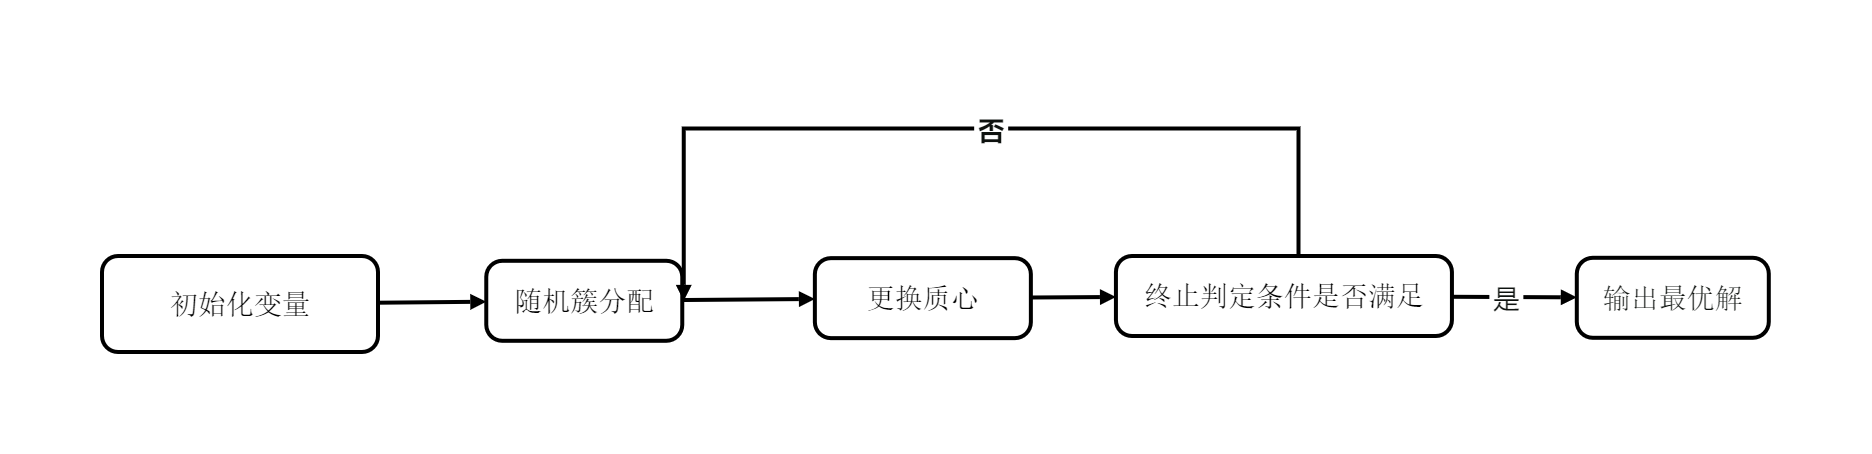
\includegraphics[width=0.8\textwidth]{image17.png}  % 将宽度增加至 80% 的页面宽度
		\caption{聚类分析流程图}
		\label{fig:yield_comparison1}
	\end{figure}
	本题使用聚类分析法求解最优值
	\subsubsection{数据输入}
	给定一个包含 n 个元素的集合 $X=\left(x_1, x_2, x_3, \ldots, x_n\right)$,
	每个数据点 $x_i \in \mathbb{R}^d$ 是 d 维向量
	\subsubsection{定义聚类中心}
	寻找 k 个簇的中心, 用向量
	 \begin{equation}\vec{K}=\left(k_1, k_2, k_3, \ldots, k_k\right)\end{equation}
	 
	 表示
	\subsubsection{初始化}
	从数据集 $X$ 中随机选择 k 个点作为初始质心
	\subsubsection{簇分配}
	在每次迭代中,根据当前质心的空间坐标,将每个数据点分配给最近的质心。定义 $c_i$ 为数据点 $x_i$ 所分配的第 j 个簇的索引, $\mu_j$ 为第 j 个簇的质心, 则有:
\begin{equation}
	c_i=\operatorname{argmin}_j\left\|x_i-\mu_j\right\|^2
\end{equation}
	\subsubsection{质心更新}
	定义 $C_j$ 是第 j 个簇的点集, 计算当前簇中所有数据点的均值
	 \begin{equation}\mu_j=\frac{1}{\left|C_j\right|} \cdot \sum x_i \in C_j x_i
	 \end{equation}
	 
	 
	将下一步质心的位置设定为均值 $\mu_j$
	\subsubsection{目标函数}
	目标函数是最小化所有数据点与其对应质心的欧氏距离总和。
\begin{equation}
	\text { 令 } J=\sum_{i=1}^n\left\|x_i-\mu_{C_i}\right\|^2
\end{equation}

	$\mu_{C_i}$ 是分配给数据点 $x_i$ 的质心
	\subsubsection{算法终止判定}
\begin{equation}
	\left(\mu_{C_i}^{\text {new }}=\mu_{C_i}\right) \vee\left(\lim _{i \rightarrow+\infty} J=\varepsilon, \varepsilon \in \mathbb{R}\right)
\end{equation}


	\subsubsection{结果输出}
	
	
	  根据农作物经济学指标聚类图可知,在亩产量-种植成本平面上存在部分呈现较强正相关性的农作物,意味着这部分作物的亩产量会随着种植成本的提升而增大。这一部分作物可进一步聚类为两个簇,在每个簇的置信空间内,作物之间在培育策略上具有较强可替代性。
	  \newline
		\begin{figure}[h]
		\centering
		\begin{minipage}{0.48\textwidth}
			\centering
			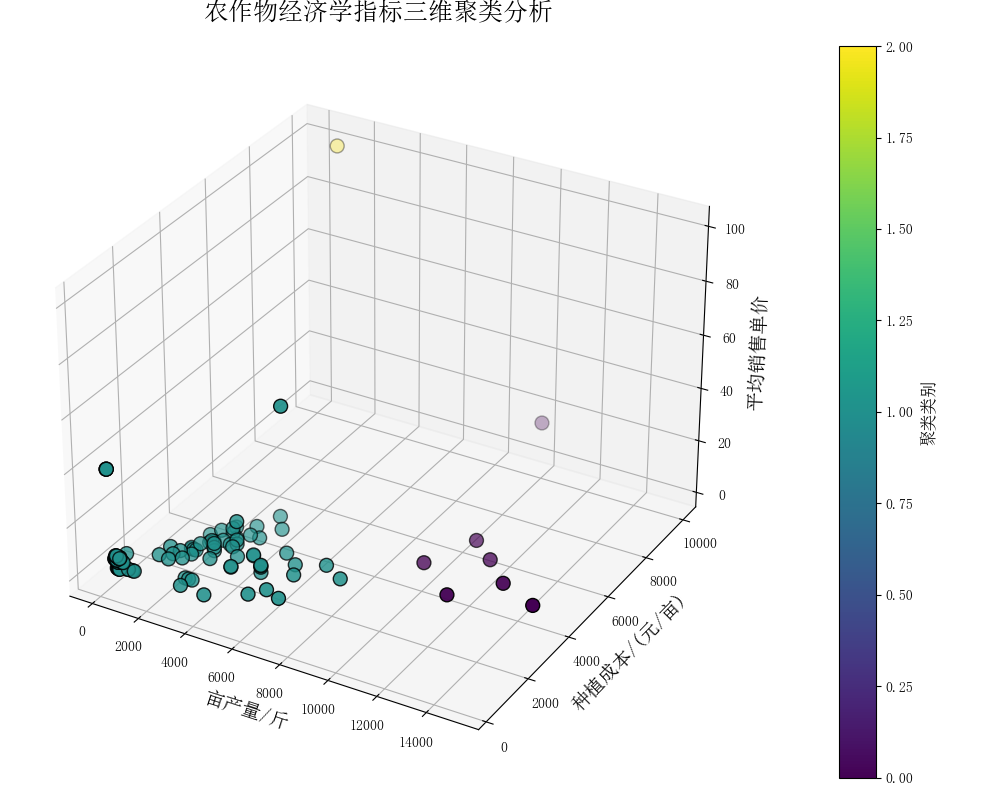
\includegraphics[width=\linewidth]{image12.png}
			\caption{农作物经济学指标聚类图1}
			\label{fig:yield_comparison1}
		\end{minipage}\hfill
		\begin{minipage}{0.48\textwidth}
			\centering
			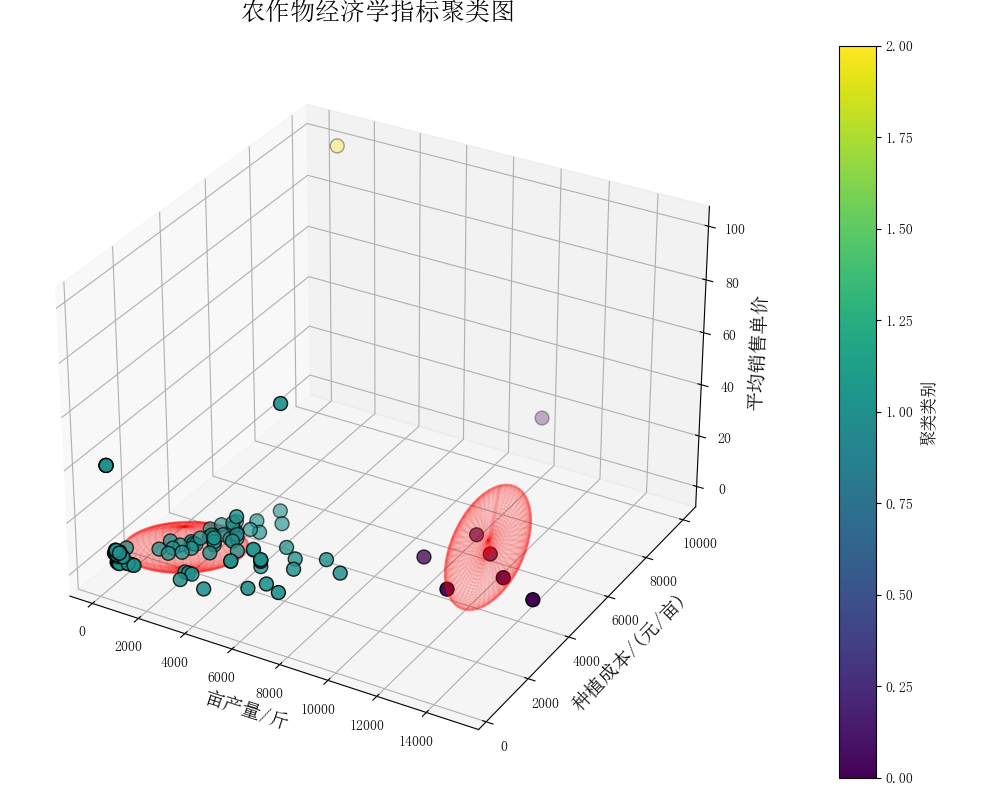
\includegraphics[width=\linewidth]{image11.png}
			\caption{农作物经济学指标聚类图2}
			\label{fig:yield_comparison2}
		\end{minipage}
	\end{figure}
	
	
	这意味着簇内某种作物因自然灾害等不可抗因素影响下无法获得收益时,可以用簇内其他的农作物替代该作物取得最优收益,维持生产效益。

\newpage
	\subsection{比较分析}
	
	
	在第三问的条件下, 可知在作物可替换情况下, 干旱地, 梯田和山坡地相比第二问变为了偶数年以红薯为主要经济作物, 奇数年以荞麦为主要经济作物。水浇地则变为偶数年水稻茄子双季种植, 奇数年第一季种植茄子与豇豆, 第二季种植水稻。普通大棚则两季主要种植豇豆,辅种刀豆。智慧大棚单季则以茄子为主要粮食作物, 约占总量的百分之六十, 其余粮食作物主要则种植土豆与西红柿, 双季则种植豆类, 以豆豆为主, 约占百分之七十, 其余种植刀豆,约占百分之四十。按照此种植策略可使农产品的经济效益达到最优。
	
	
	\begin{table}[htbp]
		\centering
		\begin{tabular}{m{5cm} m{5cm} m{6cm}}  
			\toprule  
			地块类型 & 年份 & 种植作物及其比例\\  
			\midrule  
			A平旱地 & 偶数年 & 红薯 90\%, 其余 10\%\\  
			B梯田 & 偶数年& 红薯 90\%, 其余 10\%\\  
			C山坡地  & 偶数年&  红薯 90\%, 其余 10\%\\
			D 水浇地 & 偶数年第一季 & 茄子 100\% \\
			D 水浇地 & 偶数年第二季 & 水稻 100\% \\
			E 普通大棚 & 第一季 & 豇豆 90\%, 刀豆 10\% \\
			E 普通大棚 & 第二季 & 豇豆 100\% \\
			F 智慧大棚 & 第一季 & 茄子 60\%, 土豆 20\%, 西红柿20\% \\
			F 智慧大棚 & 第二季 & 豇豆 70\%, 刀豆 30\% \\
			\bottomrule  
		\end{tabular}  
		\caption{种植策略1}
	\end{table}
	
	\vspace{-0.5cm} % 减少竖直间距
	

	\begin{table}[htbp]
		\centering
		\begin{tabular}{m{5cm} m{5cm}m{6cm}}  
			\toprule  
			地块类型 & 年份 & 种植作物及其比例\\  
			\midrule  
			A平旱地 & 奇数年 & $90 \%$ 荞麦, 其余 $10 \%$ \\
			B梯田 & 奇数年 & $90 \%$ 荞麦, 其余 $10 \%$ \\
			C山坡地 & 奇数年 & $90 \%$ 荞麦, 其余 $10 \%$ \\
			D水浇地 & 奇数年第一季 & $70 \%$ 茄子, 豇豆 $30 \%$ \\
			D水浇地 & 奇数年第二季 & $100 \%$ 水稻 \\
			\bottomrule  
		\end{tabular}  
		\caption{种植策略2}
	\end{table}
	
	\section{模型的检验}  
	\label{sec:validation}  
	本题是基于预测变量正态分布假设的单目标多约束优化问题, 最重要的就是从多方面综合验证模型假设的合理性。上文中我们采用了残差分析法, 通过残差 Q-Q 图分析得出了假设在残差分位数角度合理的结论。但是上述算法均未在全局角度量化模型假设和实际波动的偏差。因此, 我们在此补充全局的残差 P-P 图分析以进一步验证模型假设和全局波动的拟合度。
	
	和之前一样我们在题目给定的的作物售价范围内随机生成价格序列, 记作 $\vec{x}=$ $\left(x_1, x_2, x_3, \ldots, x_n\right)$
	
	接着, 我们使用对数收益正态分布模型生成同等数量的服从正态分布的随机价格序列,记作 $\vec{X}=\left(X_1, X_2, X_3, \ldots, X_n\right)$, 计算得残差向量 $\vec{x}-\vec{X}=\vec{e}=\left(e_1, e_2, e_3, \ldots, e_n\right)$ 。接下来本文进行全局理论分布残差检验并绘制残差 P-P 散点图。
	
	其中 P-P 图横坐标表示正态分布累积概率, 纵坐标表示模拟生成的数据样本累积概率。理论上,散点图拟合曲线越逼近 $y=x$ 的参考线,说明数据分布越符合理论概率分布。
	
	从数据可视化角度出发, 为定量评估残差 P-P 散点图的点是否接近对角线, 我们选择单样本 K-S 检验, 步骤如下:
	
	
	\textbf{1.提出假设}
	
	原假设 $H_0$ :样本数据分布服从正态分布
	备择假设 $H_1$ :样本数据不服从正态分布
	
	
	\textbf{2. 分别计算理论分布的累积分布函数} $F\left(X_i\right)$ 和样本数据的累积分布函数 $F\left(x_i\right)$
	
	$$
	\begin{aligned}
		& F\left(X_i\right)=P\left(X_i<X\right) \\
		& F\left(x_i\right)=P\left(x_i<x\right)
	\end{aligned}
	$$
	
	\textbf{3. 计算 K-S 统计量 $D_n$}
	
	$$
	D_n=\sup _x\left|F\left(X_i\right)-F\left(x_i\right)\right|
	$$
	
	$\sup _x$ 表示对于所有 $x$,取 $\left|F\left(X_i\right)-F\left(x_i\right)\right|$ 的较大值
	
	
	\textbf{4.确定 K-S 统计量临界值}
	
	在显著性水平 $\alpha=0.05$ 条件下, 查表得到 K-S 统计量临界值 $D_\alpha$ 5.做出决策
	
	$$
	\begin{aligned}
		& D_n<D_\alpha \text { ,接收 } H_0 \text { ,拒绝 } H_1 \\
		& D_n>D_\alpha \text { ,接收 } H_1 \text { ,拒绝 } H_0
	\end{aligned}
	$$
	
	
	\textbf{灵敏度分析:}
	
	
	我们采用局部敏感性分析,基于偏导数的分析,一次分析一个参数,例如农作物的种类,农作物的价格对成本函数的影响,同时保持其他参数不变。在改变了系统参数农作物的价格后,我们发现引起这个摸型输出的变化的程度不大,如图,则说明模型灵敏性较差,即稳定性较好。农作物种类G改变了$1\% ,\mathrm{t}$ 仅下降 $3.5\%$ ,这个改变很小,可以说明模型较为稳定.
	
	本题经计算得到 $D_n<D_\alpha$, 说明在全局上模型假设在显著性水平 $\alpha=0.05$ 条件下成立。
	
	
	
	
	
	
	
	
	
	
	
	\section{模型的评价与改进}  
	\label{sec:evaluation}  
	\subsection{模型的优点:}	
	
	(1) 在第二问中引入经济学中的几何布朗运动的概念和对数收益正态分布模型, 使模型具有较高的可信度,对实际应用具有普适性。
		\begin{figure}[h]
		\centering
		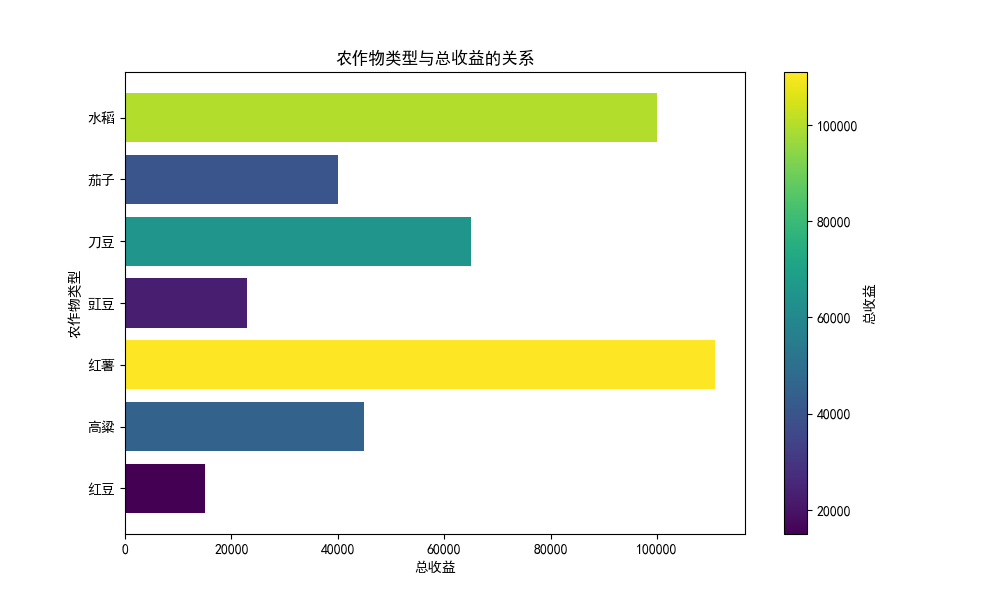
\includegraphics[width=0.8\textwidth]{image16.png}  % 将宽度增加至 80% 的页面宽度
		\caption{不同农作物类型与总收益的关系}
		\label{fig:yield_comparison1}
	\end{figure}
	
	(2)针对本题的要求采用了遗传算法进行优化,有效地解决了约束条件非线性的问题,且计算结果准确。
	
	
	(3)考虑到本题的样本较少,采用鲁棒优化模型可以更好接近不同情境下的最优解,同时可以进一步改造遗传算法,提高优化效率。
	\subsection{模型的缺点:}	
	(1)使用遗传算法有时只能得出局部最优解而非全局最优解。必须通过多次模拟才能得出较为可靠的结论。
	
	
	(2)在问题 2 求解中,时间复杂度较高导致求解效率低。
	\subsection{模型的改进:}	
	(1)考虑作物生长周期内的动态变化,引入时间序列分析,考虑作物生长周期内(如季度、年度) 的价格、销量、成本等关键指标的动态变化, 提高种植决策的灵活性和适应性。
	
	
	(2)除了考虑农作物的经济收益外, 结合多种因素实现多目标优化, 使模型更加可信。  
	
	
	
	
	\newpage
%\section*{参考文献}  
\begin{thebibliography}{9} % {9}表示参考文献编号的最大宽度,根据实际需要调整  
	
	\bibitem{[1]} 陈静, 李磊, 倪明放. 基于几何布朗运动的投资组合模型[J]. 数学的实践与认识, 2008, (17): 24-27.   
	
	
	\bibitem{[2]} 司守奎, 孙兆亮. 数学建模算法与应用[M]. 第2版. 北京: 国防工业出版社, 2016.  
	
	
	\bibitem{[3]}段玉倩,贺家李.遗传算法及其改进[J].电力系统及其自动化学报,1998,(01):43-56.
	
	\bibitem{[4]}寿涌毅,王伟.基于鲁棒优化模型的项目调度策略遗传算法[J].管理工程学报,2009,23(04):148-152.
	
	\bibitem{[5]}张建萍,刘希玉.基于聚类分析的K-means算法研究及应用[J].计算机应用研究,2007,(05):166-168.
	
	\bibitem{[6]}陈静,李磊,倪明放.基于几何布朗运动的投资组合模型[J].数学的实践与认识,2008,(17):24-27.
\end{thebibliography} 
	 
	 
	 \newpage
	\section*{附录}  
	\subsection*{附录1 支撑材料}
	\label{sec:appendix}  
	\appendix
\begin{table}[htbp]
	\centering
	\begin{tabular}{m{5cm} m{10cm}}  
		\toprule  
		符号 & 符号含义\\  
		\midrule  
		result1\_1.xlsx & 问题一第一小问求解结果\\  
		result1\_2.xlsx & 问题一第二小问求解结果\\  
		result2.xlsx   & 问题二求解结果\\
		问题一第一问.py & 问题一第一小问程序\\
		问题一第二问.py & 问题一第二小问程序\\
		问题二.py & 问题二程序\\
		问题三.py & 问题三程序\\
		问题三可视化.py & 问题三可视化绘图程序\\
		遗传算法.py & 问题一遗传算法算法程序\\
		线性规划.py & 标准线性规划程序\\
		聚类分析.py & 问题三聚类分析算法程序\\
		条形图.py & 数据可视化程序\\
		轮作约束.py & 问题约束代码\\
		相关性分析.py & 问题三相关性分析程序\\
		附件1.xlsx & 题目修改后的附件1\\
		附件2.xlsx & 题目修改后的附件2\\
		附件3.xlsx & 题目修改后的附件3\\
		中间数据.csv & 中间数据\\
	%	$V$ & 蔬菜的集合\\
	%	$B$ & 豆类的集合\\
	%	$m$ & 地块数量\\
	%	$n$ & 农作物种类数量\\
		\bottomrule  
	\end{tabular}  
%	\caption{符号及其含义}
\end{table}
 
 \newpage
 
	\section{问题一第一小问代码}  
	\noindent 
	\begin{verbatim}
		import pulp
		import pandas as pd
 
	\end{verbatim}
	
	
	\section{问题一第二小问代码}  
	\noindent 
	\begin{verbatim}
		import pulp
		import pandas as pd
		
		# 读取用户上传的数据
		file_path = '附件1.xlsx'
		file_path_2 = '附件2.xlsx'
		file_path_3 = '附件3.xlsx'
		df_land = pd.read_excel(file_path, sheet_name='乡村的现有耕地')
		df_crops = pd.read_excel(file_path_2, sheet_name='2023年统计的相关数据')
		df_sells = pd.read_excel(file_path_3)
		
		# 定义豆类作物的编号集合
		bean_crops = {1, 2, 3, 4, 5, 17, 18, 19}
		
		# 整理地块类型并分类
		A = {row['地块名称']: row['地块面积/亩'] for _, row in df_land.iterrows()}
		
		# 计算预期销售量 = 地块面积 * 亩产量
		expected_sales = {row['作物编号']: row['产量合计'] for _, 
			row in df_sells.iterrows()}
		
		# 单季地块:平旱地、梯田、山坡地
		plots_single_season = df_land[df_land['地块类型'].isin(['平旱地', 
		'梯田', '山坡地'])]['地块名称'].tolist()
		
		# 双季地块:水浇地、普通大棚、智慧大棚
		plots_double_season = df_land[df_land['地块类型'].isin(['水浇地',
		 '普通大棚', '智慧大棚'])]['地块名称'].tolist()
		#将双季节再进行细分一下
		irrigated_land = df_land[df_land['地块类型'] == '水浇地']
		['地块名称'].tolist()
		greenhouse_land = df_land[df_land['地块类型'] == '普通大棚']
		['地块名称'].tolist()
		smart_greenhouse_land = df_land[df_land['地块类型'] == '智慧大棚']
		['地块名称'].tolist()
		# 创建问题实例
		model = pulp.LpProblem("Crop_Planting_Optimization", pulp.LpMaximize)
		
		# 定义作物类型
		crops_single_season = list(range(1, 16))  # 作物1-15,适用于单季地块
		crops_double_season_irrigated = list(range(16, 38)) 
		 # 作物16-37,适用于水浇地
		crops_double_season_greenhouse = list(range(23, 42))
		  # 作物23-41,适用于普通大棚
		crops_double_season_smart = list(range(27, 35))  
		# 作物27-34,适用于智慧大棚
		
		# 处理销售单价列,取范围的平均值
		df_crops['销售单价(元/斤)'] = df_crops['销售单价/(元/斤)'].apply(
		lambda x: (float(x.split('-')[0]) + float(x.split('-')[1])) / 2 
		if isinstance(x, str) else x
		)
		
		# 生成销售单价、亩产量和种植成本的字典
		P = {row['作物编号']: row['销售单价(元/斤)'] for _, 
			row in df_crops.iterrows()}  # 销售单价字典
		Y = {row['作物编号']: row['亩产量/斤'] for _, 
			row in df_crops.iterrows()}  # 亩产量字典
		C = {row['作物编号']: row['种植成本/(元/亩)']
			 for _, row in df_crops.iterrows()}  # 种植成本字典
		
		# 定义决策变量 x[i][k][t] 是地块 i 在年份 t 的季节 j 是否种植作物 k
		years = list(range(2024, 2031))  # 从2024到2030
		x = pulp.LpVariable.dicts("x", (plots_single_season
		 + plots_double_season,
		crops_single_season + crops_double_season_irrigated 
		+ crops_double_season_greenhouse + crops_double_season_smart,
		years, [1, 2]), 0, 1, cat='Continuous')
		# 定义辅助二进制变量 y1 和 y2
		y1 = pulp.LpVariable.dicts("y1", (plots_single_season
		 + plots_double_season,
		crops_single_season + crops_double_season_irrigated
		+ crops_double_season_greenhouse + crops_double_season_smart,
		years, [1, 2]), 0, 1, cat='Binary')
		
		y2 = pulp.LpVariable.dicts("y2", (plots_single_season
		 + plots_double_season,
		crops_single_season + crops_double_season_irrigated 
		+ crops_double_season_greenhouse + crops_double_season_smart,
		years, [1, 2]), 0, 1, cat='Binary')
		#新变量:超出部分的产量
		excess = pulp.LpVariable.dicts("excess", (plots_single_season 
		+ irrigated_land
		+ greenhouse_land + smart_greenhouse_land,
		crops_single_season + crops_double_season_irrigated 
		+ crops_double_season_greenhouse + crops_double_season_smart,
		years, [1, 2]), lowBound=0, cat='Continuous')
		
		# 目标函数:最大化所有地块的净收益
		# 单季地块目标函数(处理滞销和降价的情况)
		Z_single = pulp.lpSum(
		P[k] * min(Y[k] * A[i], expected_sales[k]) * x[i][k][t][1] 
		 # 正常销售收入
		+ 0.5 * P[k] * max(0, Y[k] * A[i] - expected_sales[k]) * x[i][k][t][1] 
		# 滞销部分按 50% 的价格销售
		- C[k] * A[i] * x[i][k][t][1]  # 种植成本
		for t in years 
		for i in plots_single_season 
		for k in crops_single_season
		)
		
		# 双季地块(水浇地)目标函数
		Z_irrigated = pulp.lpSum(
		P[k] * min(Y[k] * A[i], expected_sales[k]) * (x[i][k][t][1] 
		+ x[i][k][t][2])
		# 正常销售收入
		+ 0.5 * P[k] * max(0, Y[k] * A[i] - expected_sales[k]) 
		* (x[i][k][t][1] + x[i][k][t][2]) 
		# 滞销部分按 50% 的价格销售
		- C[k] * A[i] * (x[i][k][t][1] + x[i][k][t][2])  # 种植成本
		for t in years
		for i in irrigated_land
		for k in crops_double_season_irrigated
		)
		
		# 普通大棚目标函数
		Z_greenhouse = pulp.lpSum(
		P[k] * min(Y[k] * A[i], expected_sales[k]) * (x[i][k][t][1]
		 + x[i][k][t][2])  
		# 正常销售收入
		
		+ 0.5 * P[k] * max(0, Y[k] * A[i] - expected_sales[k]) 
		* (x[i][k][t][1] + x[i][k][t][2]) 
		# 滞销部分按 50% 的价格销售
		- C[k] * A[i] * (x[i][k][t][1] + x[i][k][t][2])  # 种植成本
		for t in years
		for i in greenhouse_land
		for k in crops_double_season_greenhouse
		)
		
		# 智慧大棚目标函数
		Z_smart_greenhouse = pulp.lpSum(
		P[k] * min(Y[k] * A[i], expected_sales[k]) 
		* (x[i][k][t][1] + x[i][k][t][2])
		# 正常销售收入
		+ 0.5 * P[k] * max(0, Y[k] * A[i] - expected_sales[k]) 
		* (x[i][k][t][1] + x[i][k][t][2])
		# 滞销部分按 50% 的价格销售
		- C[k] * A[i] * (x[i][k][t][1] + x[i][k][t][2])  # 种植成本
		for t in years
		for i in smart_greenhouse_land
		for k in crops_double_season_smart
		)
		
		# 综合目标函数
		model += Z_single + Z_irrigated + Z_greenhouse
		 + Z_smart_greenhouse
		def objective_case2():
		return pulp.lpSum(
		P[k] * Y[k] * x[i][k][t][j]  # 正常销售收入
		- P[k] * excess[i][k][t][j]  # 滞销部分(正常价格销售的部分减少)
		+ 0.5 * P[k] * excess[i][k][t][j]  # 降价销售的部分
		- C[k] * x[i][k][t][j]  # 种植成本
		for t in years
		for i in plots_single_season + irrigated_land + greenhouse_land 
		+ smart_greenhouse_land
		for k in crops_single_season + crops_double_season_irrigated 
		+ crops_double_season_greenhouse + crops_double_season_smart
		for j in [1, 2]
		)
		
		
		#x变量约束条件
		for i in plots_single_season + irrigated_land + greenhouse_land 
		+ smart_greenhouse_land:
		for k in crops_single_season + crops_double_season_irrigated
		+ crops_double_season_greenhouse + crops_double_season_smart:
		for t in years:
		for j in [1, 2]:
		# 约束 x 的值等于 0.5 * y1 + y2
		model += x[i][k][t][j] == 0.5 * y1[i][k][t][j] + y2[i][k][t][j]
		# 确保 y1 和 y2 不会同时为 1
		model += y1[i][k][t][j] + y2[i][k][t][j] <= 1
		# 约束条件1:为每种地块类型添加作物选择约束
		for t in years:
		# 单季地块(平旱地、梯田、山坡地)限制作物选择
		for i in plots_single_season:
		# 在每年只能从作物 {1, 2, ..., 15} 中选择
		model += pulp.lpSum(x[i][k][t][1] for k in crops_single_season) == 1
		# 双季地块
		# 水浇地
		for i in irrigated_land:
		# 第一季可以在 {16, 17, ..., 34} 中选择
		model += pulp.lpSum(x[i][k][t][1] for k in range(16, 35)) == 1
		# 第二季只能在 {16, 35, 36, 37} 中选择
		model += pulp.lpSum(x[i][k][t][2] for k in [16, 35, 36, 37]) == 1
		
		# 普通大棚
		for i in greenhouse_land:
		# 第一季可以在 {17, 18, ..., 34} 中选择
		model += pulp.lpSum(x[i][k][t][1] for k in range(17, 35)) == 1
		# 第二季只能在 {38, 39, 40, 41} 中选择
		model += pulp.lpSum(x[i][k][t][2] for k in range(38, 42)) == 1
		
		# 智慧大棚
		for i in smart_greenhouse_land:
		# 第一季和第二季都只能在 {17, 18, ..., 34} 中选择
		model += pulp.lpSum(x[i][k][t][1] for k in range(17, 35)) == 1
		model += pulp.lpSum(x[i][k][t][2] for k in range(17, 35)) == 1
		
		# 约束条件2:在每块地上每季的作物种植比例之和为1
		for t in years:
		for i in plots_single_season:
		model += pulp.lpSum(x[i][k][t][1] for k in crops_single_season) == 1
		
		for i in plots_double_season:
		for j in [1, 2]:
		model += pulp.lpSum(x[i][k][t][j] for k in crops_double_season_irrigated
		+ crops_double_season_greenhouse + crops_double_season_smart) == 1
		
		# 约束条件3:轮作约束
		for t in years[:-1]: 
		for i in plots_single_season:
		for k in crops_single_season:
		model += y1[i][k][t][1] + y2[i][k][t][1] + y1[i][k][t+1][1] 
		+ y2[i][k][t+1][1] <= 1
		
		#对于双季地块
		for t in years[:-1]: 
		for i in irrigated_land + greenhouse_land + smart_greenhouse_land:
		for k in crops_double_season_irrigated + crops_double_season_greenhouse
		+ crops_double_season_smart:
		model += y1[i][k][t][1] + y2[i][k][t][1] + y1[i][k][t][2] 
		+ y2[i][k][t][2] <= 1
		model += y1[i][k][t][2] + y2[i][k][t][2] + y1[i][k][t+1][1]
		 + y2[i][k][t+1][1] <= 1
		
		# 求解模型
		model.solve()
		
		# 创建一个空列表来存储结果
		results = []
		
		# 遍历所有变量,并将非零决策变量的值保存下来
		for i in plots_single_season + plots_double_season:
		for k in crops_single_season + crops_double_season_irrigated 
		+ crops_double_season_greenhouse + crops_double_season_smart:
		for t in years:
		for j in [1, 2]:
		if x[i][k][t][j].varValue is not None and x[i][k][t][j].varValue > 0:
		results.append([i, k, t, j, x[i][k][t][j].varValue])
		
		# 使用 pandas 将结果转换为数据框
		df_results = pd.DataFrame(results, columns=["地块",
		 "作物", "年份", "季节", "种植比例"])
		
		# 显示结果
		print(df_results)
		output_path = "optimization_results4.csv"
		# df_results.to_csv(output_path, index=False)
		# print("保存成功!")
	\end{verbatim}
	
	%\section{问题代码}  
	
	\noindent 
	\section{问题二代码}
	\begin{verbatim}
		import pulp
		import pandas as pd
		import numpy as np
		
		# 读取用户上传的数据
		file_path = '附件1.xlsx'
		df_land = pd.read_excel(file_path, sheet_name='乡村的现有耕地')
		
		file_path_2 = '附件2.xlsx'  # 确保路径指向正确的文件
		df_crops = pd.read_excel(file_path_2, sheet_name='2023年统计的相关数据')
		
		# 定义豆类作物的编号集合
		bean_crops = {1, 2, 3, 4, 5, 17, 18, 19}
		
		# 整理地块类型并分类
		A = {row['地块名称']: row['地块面积/亩'] for _, row in df_land.iterrows()}
		
		# 单季地块:平旱地、梯田、山坡地
		plots_single_season = df_land[df_land['地块类型'].isin(['平旱地', '梯田', '山坡地'])]['地块名称'].tolist()
		
		# 双季地块:水浇地、普通大棚、智慧大棚
		plots_double_season = df_land[df_land['地块类型'].isin(['水浇地', '普通大棚', '智慧大棚'])]['地块名称'].tolist()
		#将双季节再进行细分一下
		irrigated_land = df_land[df_land['地块类型'] == '水浇地']['地块名称'].tolist()
		greenhouse_land = df_land[df_land['地块类型'] == '普通大棚']['地块名称'].tolist()
		smart_greenhouse_land = df_land[df_land['地块类型'] == '智慧大棚']['地块名称'].tolist()
		
		model = pulp.LpProblem("Crop_Planting_Optimization", pulp.LpMaximize)
		# 定义作物类型
		crops_single_season = list(range(1, 16))  # 作物1-15,适用于单季地块
		crops_double_season_irrigated = list(range(16, 38))  # 作物16-37,适用于水浇地
		crops_double_season_greenhouse = list(range(23, 42))  # 作物23-41,适用于普通大棚
		crops_double_season_smart = list(range(27, 35))  # 作物27-34,适用于智慧大棚
		
		# 处理销售单价列,取范围的平均值
		df_crops['销售单价(元/斤)'] = df_crops['销售单价/(元/斤)'].apply(
		lambda x: (float(x.split('-')[0]) + float(x.split('-')[1])) / 2 if isinstance(x, str) else x
		)
		
		# 生成销售单价、亩产量和种植成本的字典
		P = {row['作物编号']: row['销售单价(元/斤)'] for _, row in df_crops.iterrows()}  # 销售单价字典
		Y = {row['作物编号']: row['亩产量/斤'] for _, row in df_crops.iterrows()}  # 亩产量字典
		C = {row['作物编号']: row['种植成本/(元/亩)'] for _, row in df_crops.iterrows()}  # 种植成本字典
		
		# 定义波动范围
		price_uncertainty = 0.1  # 销售单价波动范围 ±10%
		yield_uncertainty = 0.1  # 亩产量波动范围 ±10%
		cost_uncertainty = 0.05  # 种植成本波动范围 ±5%
		
		# 定义决策变量 x[i][k][t] 是地块 i 在年份 t 的季节 j 是否种植作物 k(取值为0, 0.5或1)
		years = list(range(2024, 2031))  # 从2024到2030
		x = pulp.LpVariable.dicts("x", (plots_single_season + plots_double_season,
		crops_single_season + crops_double_season_irrigated
		+ crops_double_season_greenhouse + crops_double_season_smart,
		years, [1, 2]), 0, 1, cat='Continuous')
		
		# 定义辅助二进制变量 y1 和 y2
		y1 = pulp.LpVariable.dicts("y1", (plots_single_season + plots_double_season,
		crops_single_season + crops_double_season_irrigated 
		+ crops_double_season_greenhouse + crops_double_season_smart,
		years, [1, 2]), 0, 1, cat='Binary')
		
		y2 = pulp.LpVariable.dicts("y2", (plots_single_season + plots_double_season,
		crops_single_season + crops_double_season_irrigated 
		+ crops_double_season_greenhouse + crops_double_season_smart,
		years, [1, 2]), 0, 1, cat='Binary')
		
		# 单季地块目标函数(稳健优化)
		Z_single = pulp.lpSum(
		((P[k] * (1 - price_uncertainty) * Y[k] * (1 - yield_uncertainty) * A[i] 
		# 销售收入 (销售价格和亩产量的不确定性)
		- C[k] * (1 + cost_uncertainty) * A[i])  # 种植成本 (种植成本的不确定性)
		* x[i][k][t][1])
		for t in years 
		for i in plots_single_season 
		for k in crops_single_season
		)
		
		# 双季地块(水浇地)目标函数(稳健优化)
		Z_irrigated = pulp.lpSum(
		((P[k] * (1 - price_uncertainty) * Y[k] * (1 - yield_uncertainty) * A[i] 
		# 销售收入 (销售价格和亩产量的不确定性)
		- C[k] * (1 + cost_uncertainty) * A[i])  # 种植成本 (种植成本的不确定性)
		* (x[i][k][t][1] + x[i][k][t][2]))
		for t in years
		for i in irrigated_land
		for k in crops_double_season_irrigated
		)
		
		# 普通大棚目标函数(稳健优化)
		Z_greenhouse = pulp.lpSum(
		((P[k] * (1 - price_uncertainty) * Y[k] * (1 - yield_uncertainty) * A[i] 
		# 销售收入 (销售价格和亩产量的不确定性)
		- C[k] * (1 + cost_uncertainty) * A[i])  # 种植成本 (种植成本的不确定性)
		* (x[i][k][t][1] + x[i][k][t][2]))
		for t in years
		for i in greenhouse_land
		for k in crops_double_season_greenhouse
		)
		
		# 智慧大棚目标函数(稳健优化)
		Z_smart_greenhouse = pulp.lpSum(
		((P[k] * (1 - price_uncertainty) * Y[k] * (1 - yield_uncertainty) * A[i] 
		# 销售收入 (销售价格和亩产量的不确定性)
		- C[k] * (1 + cost_uncertainty) * A[i])  # 种植成本 (种植成本的不确定性)
		* (x[i][k][t][1] + x[i][k][t][2]))
		for t in years
		for i in smart_greenhouse_land
		for k in crops_double_season_smart
		)
		
		
		#综合目标函数
		model += Z_single + Z_irrigated + Z_greenhouse + Z_smart_greenhouse
		
		# x变量约束条件
		for i in plots_single_season + irrigated_land + greenhouse_land 
		+ smart_greenhouse_land:
		for k in crops_single_season + crops_double_season_irrigated
		+ crops_double_season_greenhouse + crops_double_season_smart:
		for t in years:
		for j in [1, 2]:
		# 约束 x 的值等于 0.5 * y1 + y2
		model += x[i][k][t][j] == 0.5 * y1[i][k][t][j] + y2[i][k][t][j]
		# 确保 y1 和 y2 不会同时为 1
		model += y1[i][k][t][j] + y2[i][k][t][j] <= 1
		
		# 约束条件1:为每种地块类型添加作物选择约束
		for t in years:
		# 单季地块(平旱地、梯田、山坡地)限制作物选择
		for i in plots_single_season:
		model += pulp.lpSum(x[i][k][t][1] for k in crops_single_season) == 1
		
		# 双季地块(水浇地、普通大棚、智慧大棚)限制作物选择
		for i in irrigated_land:
		model += pulp.lpSum(x[i][k][t][1] for k in range(16, 35)) == 1
		model += pulp.lpSum(x[i][k][t][2] for k in [16, 35, 36, 37]) == 1
		
		for i in greenhouse_land:
		model += pulp.lpSum(x[i][k][t][1] for k in range(17, 35)) == 1
		model += pulp.lpSum(x[i][k][t][2] for k in range(38, 42)) == 1
		
		for i in smart_greenhouse_land:
		model += pulp.lpSum(x[i][k][t][1] for k in range(17, 35)) == 1
		model += pulp.lpSum(x[i][k][t][2] for k in range(17, 35)) == 1
		
		# 约束条件2:每块地每季作物种植比例之和为1
		for t in years:
		for i in plots_single_season:
		model += pulp.lpSum(x[i][k][t][1] for k in crops_single_season) == 1
		
		for i in plots_double_season:
		for j in [1, 2]:
		model += pulp.lpSum(x[i][k][t][j] for k in crops_double_season_irrigated 
		+ crops_double_season_greenhouse + crops_double_season_smart) == 1
		
		# 约束条件3:轮作约束
		for t in years[:-1]: 
		for i in plots_single_season:
		for k in crops_single_season:
		model += y1[i][k][t][1] + y2[i][k][t][1] + y1[i][k][t+1][1]
		+ y2[i][k][t+1][1] <= 1
		
		#对于双季地块
		for t in years[:-1]: 
		for i in irrigated_land + greenhouse_land + smart_greenhouse_land:
		for k in crops_double_season_irrigated + crops_double_season_greenhouse
		+ crops_double_season_smart:
		model += y1[i][k][t][1] + y2[i][k][t][1] + y1[i][k][t][2] 
		+ y2[i][k][t][2] <= 1
		model += y1[i][k][t][2] + y2[i][k][t][2] + y1[i][k][t+1][1] 
		+ y2[i][k][t+1][1] <= 1
		
		
		for t_start in range(2024, 2028):
		for i in plots_single_season:
		model += pulp.lpSum(x[i][k][t][1] 
		for k in bean_crops for t in range(t_start, t_start + 3)) >= 1
		
		for i in irrigated_land + greenhouse_land + smart_greenhouse_land:
		model += pulp.lpSum(x[i][k][t][1] + x[i][k][t][2] 
		for k in bean_crops for t in range(t_start, t_start + 3)) >= 1
		
		# 求解模型
		model.solve()
		
		# 创建一个空列表来存储结果
		results = []
		
		# 遍历所有变量,并将非零决策变量的值保存下来
		for i in plots_single_season + plots_double_season:
		for k in crops_single_season + crops_double_season_irrigated + crops_double_season_greenhouse
		 + crops_double_season_smart:
		for t in years:
		for j in [1, 2]:
		if x[i][k][t][j].varValue is not None and x[i][k][t][j].varValue > 0:
		results.append([i, k, t, j, x[i][k][t][j].varValue])
		
		# 使用 pandas 将结果转换为数据框
		df_results = pd.DataFrame(results, columns=["地块", "作物", "年份", "季节", "种植比例"])
		
		# 显示结果
		print(df_results)
	\end{verbatim}
	\noindent
	\section{问题三代码}
	\begin{verbatim}
		import pulp
		import pandas as pd
		
		file_path = '附件1.xlsx'
		df_land = pd.read_excel(file_path, sheet_name='乡村的现有耕地')
		
		file_path_2 = '附件2.xlsx' 
		df_crops = pd.read_excel(file_path_2, sheet_name='2023年统计的相关数据')
		
		bean_crops = {1, 2, 3, 4, 5, 17, 18, 19}
		
		A = {row['地块名称']: row['地块面积/亩'] for _, row in df_land.iterrows()}
		
		plots_single_season = df_land[df_land['地块类型'].isin(['平旱地', '梯田', '山坡地'])]['地块名称'].tolist()
		
		plots_double_season = df_land[df_land['地块类型'].isin(['水浇地', '普通大棚', '智慧大棚'])]
		['地块名称'].tolist()
		
		irrigated_land = df_land[df_land['地块类型'] == '水浇地']['地块名称'].tolist()
		greenhouse_land = df_land[df_land['地块类型'] == '普通大棚']['地块名称'].tolist()
		smart_greenhouse_land = df_land[df_land['地块类型'] == '智慧大棚']['地块名称'].tolist()
		
		model = pulp.LpProblem("Crop_Planting_Optimization", pulp.LpMaximize)
		
		crops_single_season = list(range(1, 16))  # 作物1-15,适用于单季地块
		crops_double_season_irrigated = list(range(16, 38))  # 作物16-37,适用于水浇地
		crops_double_season_greenhouse = list(range(23, 42))  # 作物23-41,适用于普通大棚
		crops_double_season_smart = list(range(27, 35))  # 作物27-34,适用于智慧大棚
		
		df_crops['销售单价(元/斤)'] = df_crops['销售单价/(元/斤)'].apply(
		lambda x: (float(x.split('-')[0]) + float(x.split('-')[1])) / 2 if isinstance(x, str) else x
		)
		
		P = {row['作物编号']: row['销售单价(元/斤)'] for _, row in df_crops.iterrows()}  # 销售单价字典
		Y = {row['作物编号']: row['亩产量/斤'] for _, row in df_crops.iterrows()}  # 亩产量字典
		C = {row['作物编号']: row['种植成本/(元/亩)'] for _, row in df_crops.iterrows()}  # 种植成本字典
		
		years = list(range(2024, 2031))  # 从2024到2030
		x = pulp.LpVariable.dicts("x", (plots_single_season + plots_double_season,
		crops_single_season + crops_double_season_irrigated + crops_double_season_greenhouse
		 + crops_double_season_smart,
		years, [1, 2]), 0, 1, cat='Continuous')
		y1 = pulp.LpVariable.dicts("y1", (plots_single_season + plots_double_season,
		crops_single_season + crops_double_season_irrigated + crops_double_season_greenhouse 
		+ crops_double_season_smart,
		years, [1, 2]), 0, 1, cat='Binary')
		
		y2 = pulp.LpVariable.dicts("y2", (plots_single_season + plots_double_season,
		crops_single_season + crops_double_season_irrigated + crops_double_season_greenhouse 
		+ crops_double_season_smart,
		years, [1, 2]), 0, 1, cat='Binary')
		
		# 目标函数:最大化所有地块的净收益
		# 单季地块目标函数
		# 单季地块目标函数
		Z_single = pulp.lpSum(
		(P[k] * Y[k] * A[i] - C[k] * A[i]) * x[i][k][t][1] 
		for t in years 
		for i in plots_single_season 
		for k in crops_single_season
		)
		
		# 双季地块目标函数
		Z_irrigated = pulp.lpSum(
		(P[k] * Y[k] * A[i] - C[k] * A[i]) * (x[i][k][t][1] + x[i][k][t][2])
		for t in years
		for i in irrigated_land
		for k in crops_double_season_irrigated
		)
		
		Z_greenhouse = pulp.lpSum(
		(P[k] * Y[k] * A[i] - C[k] * A[i]) * (x[i][k][t][1] + x[i][k][t][2])
		for t in years
		for i in greenhouse_land
		for k in crops_double_season_greenhouse
		)
		
		Z_smart_greenhouse = pulp.lpSum(
		(P[k] * Y[k] * A[i] - C[k] * A[i]) * (x[i][k][t][1] + x[i][k][t][2])
		for t in years
		for i in smart_greenhouse_land
		for k in crops_double_season_smart
		)
		
		model += Z_single + Z_irrigated + Z_greenhouse + Z_smart_greenhouse
		for i in plots_single_season + irrigated_land + greenhouse_land 
		+ smart_greenhouse_land:
		for k in crops_single_season + crops_double_season_irrigated
		 + crops_double_season_greenhouse 
		+ crops_double_season_smart:
		for t in years:
		for j in [1, 2]:
		
		model += x[i][k][t][j] == 0.5 * y1[i][k][t][j] + y2[i][k][t][j]
		model += y1[i][k][t][j] + y2[i][k][t][j] <= 1
		for t in years:
		for i in plots_single_season:
		model += pulp.lpSum(x[i][k][t][1] for k in crops_single_season) == 1
		for i in irrigated_land:
		model += pulp.lpSum(x[i][k][t][1] for k in range(16, 35)) == 1
		model += pulp.lpSum(x[i][k][t][2] for k in [16, 35, 36, 37]) == 1
		
		for i in greenhouse_land:
		model += pulp.lpSum(x[i][k][t][1] for k in range(17, 35)) == 1
		model += pulp.lpSum(x[i][k][t][2] for k in range(38, 42)) == 1
		
		for i in smart_greenhouse_land:
		model += pulp.lpSum(x[i][k][t][1] for k in range(17, 35)) == 1
		model += pulp.lpSum(x[i][k][t][2] for k in range(17, 35)) == 1
		
		for t in years:
		for i in plots_single_season:
		model += pulp.lpSum(x[i][k][t][1] for k in crops_single_season) == 1
		
		for i in plots_double_season:
		for j in [1, 2]:
		model += pulp.lpSum(x[i][k][t][j] for k in crops_double_season_irrigated
		 + crops_double_season_greenhouse
		 + crops_double_season_smart) == 1
		
		for t in years[:-1]: 
		for i in plots_single_season:
		for k in crops_single_season:
		model += y1[i][k][t][1] + y2[i][k][t][1] + y1[i][k][t+1][1] + y2[i][k][t+1][1] <= 1
		
		#对于双季地块
		for t in years[:-1]: 
		for i in irrigated_land + greenhouse_land + smart_greenhouse_land:
		for k in crops_double_season_irrigated + crops_double_season_greenhouse
		 + crops_double_season_smart:
		model += y1[i][k][t][1] + y2[i][k][t][1] + y1[i][k][t][2] + y2[i][k][t][2] <= 1
		model += y1[i][k][t][2] + y2[i][k][t][2] + y1[i][k][t+1][1] + y2[i][k][t+1][1] <= 1
		
		model.solve()
		
		results = []
		
		for i in plots_single_season + plots_double_season:
		for k in crops_single_season + crops_double_season_irrigated
		 + crops_double_season_greenhouse
		 + crops_double_season_smart:
		for t in years:
		for j in [1, 2]:
		if x[i][k][t][j].varValue is not None and x[i][k][t][j].varValue > 0:
		results.append([i, k, t, j, x[i][k][t][j].varValue])
		
		df_results = pd.DataFrame(results, columns=["地块", "作物", "年份", "季节", "种植比例"])
		
		print(df_results)
		output_path = "optimization_results4.csv"
		df_results.to_csv(output_path, index=False)
		print("保存成功!")
	\end{verbatim}
	
\end{document}